\documentclass[11pt,a4paper]{article}

% ============================================================================
% PACKAGES
% ============================================================================
\usepackage[utf8]{inputenc}
\usepackage[T1]{fontenc}
\usepackage{amsmath,amssymb,amsthm}
\usepackage{mathtools}
\usepackage{geometry}
\usepackage{enumitem}
\usepackage{booktabs}
\usepackage{array}
\usepackage{longtable}
\usepackage{pdflscape}
\usepackage{graphicx}
\usepackage[colorlinks=true, urlcolor=blue, linkcolor=blue, citecolor=blue]{hyperref}

\geometry{margin=1in}
\emergencystretch=1.5em
\hbadness=2500

% ============================================================================
% THEOREM ENVIRONMENTS
% ============================================================================
\theoremstyle{plain}
\newtheorem{theorem}{Theorem}[section]
\newtheorem{lemma}[theorem]{Lemma}
\newtheorem{proposition}[theorem]{Proposition}
\newtheorem{corollary}[theorem]{Corollary}

\theoremstyle{definition}
\newtheorem{definition}[theorem]{Definition}

\theoremstyle{remark}
\newtheorem{remark}[theorem]{Remark}

% ============================================================================
% CUSTOM COMMANDS
% ============================================================================
\newcommand{\N}{\mathbb{N}}
\newcommand{\Z}{\mathbb{Z}}
\newcommand{\Q}{\mathbb{Q}}
\newcommand{\R}{\mathbb{R}}
\newcommand{\C}{\mathbb{C}}
\newcommand{\F}{\mathbb{F}}
\DeclareMathOperator{\Full}{Full}
\DeclareMathOperator{\Mid}{Mid}
\DeclareMathOperator{\Prod}{Prod}
\DeclareMathOperator{\eff}{eff}
\DeclareMathOperator{\Str}{Str}
\DeclareMathOperator{\rank}{rank}

% ============================================================================
% TITLE
% ============================================================================
\title{The magnitude of the hidden constant\\in exponent-$9/4$ matrix multiplication}

\author{Luke A. D. Hutchison}

\date{\today}

% ============================================================================
% DOCUMENT
% ============================================================================
\begin{document}

\maketitle

% ============================================================================
% ABSTRACT
% ============================================================================
\begin{abstract}
In October~2026, OpenAI proved the non-constructive spectral upper bound $\omega \le 9/4$ (October~2, 2026), and Rafael Pass (\emph{Matrix Multiplication from Polynomial Packings: A Constructive Proof of $\omega \le 9/4$}, October~30, 2026) eliminated the asymptotic spectrum to give an explicit recursive $O(n^{9/4+\delta})$ algorithm for that one-sided upper bound; on November~24, 2026, OpenAI released \emph{The matrix multiplication exponent is nine fourths}, reporting the matching lower bound $\omega_{\F} = 9/4$ over every field $\F$. In Pass's Theorem~4.3, iterating polynomial packings over parameters $(c, d, k)$ yields an approximate bilinear identity on $v_k \times v_k$ matrices (the pre-Bini \emph{base block size}), and Bini $\varepsilon$-interpolation converts it into an exact rational identity of rank $R < V^\tau$ ($\tau = 9/4 + \delta$) on $V \times V$ matrices (the post-Bini \emph{base block size}, the fixed block dimension partitioned recursively as $2 \times 2$ is in Strassen's algorithm). Pass noted qualitatively that the algorithm is ``galactic'' with enormous hidden constants, without quantifying them. This paper calculates sharp universal lower bounds and matching constructive upper bounds on those constants, and proves the rigid algebraic constraints on polynomial degrees, pole orders, and tensor symmetrization that no valid realization can violate.

Even though every algebraic layer works and composing them proves $\omega \le 9/4$ mathematically, the pre-Bini base block size $v_k \times v_k$ required before the composed recursion breaks even with classical exponents is astronomical across every valid parameter choice $(c, d, k)$ of Pass's Theorem~4.3: to beat Strassen ($\tau = 2.800$), $v_k > 10^{7{,}197}$ universally (attained at $v_k \approx 10^{7{,}928}$ with $6d = 834$ variables and $k = 114$ rounds); to beat Coppersmith--Winograd ($\tau = 2.371$), $v_k > 10^{1.67 \times 10^6}$ (attained at $v_k \approx 10^{1.77 \times 10^6}$ with $6d = 20{,}352$ variables and $k = 3{,}769$ rounds); and to reach $\tau = 2.251$, $v_k > 10^{1.62 \times 10^{13}}$ (attained at $v_k \approx 10^{1.66 \times 10^{13}}$ with $6d \approx 6.16 \times 10^8$ variables and $k \approx 1.41 \times 10^8$ rounds). Those figures are before Bini $\varepsilon$-interpolation inflates the exact block side exponentially further to $V > 10^{9.51 \times 10^5}$ (attained at $10^{1.17 \times 10^6}$) at $\tau = 2.800$, $V > 10^{6.15 \times 10^9}$ (attained at $10^{6.73 \times 10^9}$) at $\tau = 2.371$, and $V > 10^{2.08 \times 10^{21}}$ (attained at $10^{2.15 \times 10^{21}}$) at $\tau = 2.251$, forcing $C(\tau) \ge (V - 1)^{3-\tau}$ in $T(n) \le C(\tau)\,n^\tau$. At any matrix size $n$ that fits in real memory, running the composed recursion directly would do vastly more work than naive $O(n^3)$.

Across all valid realizations (including Pass's entire generalized Remark~4.5 meta-family, even at zero balancing loss), these algebraic constraints lock $\log_{10} v_k(\delta) = \Theta(\delta^{-3}(\ln\delta^{-1})^2)$ and $\log_{10} V(\delta) = \Theta(\delta^{-5}(\ln\delta^{-1})^3)$. Exact balanced-word counting $M_d$ and L\"u's $(2w - 1)$-point substitution cut $\log_{10} V$ by $1.8\times$ to $5.9\times$ without altering this scaling, while single-shot untwisting of Strassen's $\Str_3$ lowers the sub-Strassen side to $10^{23.5}$ (direct sum) and $10^{343.3}$ (single matrix) before stalling at $3\log_6 4 \approx 2.32112$. Beyond polynomial packings, every border-rank realization obeying $r_0 \ge v_0^{9/4}$ satisfies the universal Bini horizon $V > (h E_\varepsilon + 1)^{1/\delta}$. Finally, we delimit the boundary for arbitrary bilinear algorithms: Pass-scale lower bounds are disproved for $\tau \in (2.32112, 3)$ by Strassen, Pan ($V = 70$), and untwisted $\Str_3$, while for $\tau \in (9/4, 2.32112)$ every supermultiplicative rank bound obeys $\Phi(V) \le V^{9/4}$ and leaves $V = O(\delta^{-4/9})$ (including $V = 16, R = 513$ at $\tau = 2.251$) consistent with $\omega = 9/4$. Every result is mechanically verified in pure-kernel Lean~4 without external libraries and checked numerically in Python.
\end{abstract}

%-------------------------------------------------------------------------------
\section{Introduction}
\label{sec:intro}
%-------------------------------------------------------------------------------

The exponent $\omega_{\F}$ of square matrix multiplication over a field $\F$ is the infimum of all real $\tau$ such that two $n \times n$ matrices over $\F$ can be multiplied using $O(n^\tau)$ scalar arithmetic operations in $\F$. In October--November~2026, a sequence of preprints pinned $\omega_{\F}$ to $9/4$ first from above (OpenAI's non-constructive upper bound on October~2~\cite{OpenAI2026Upper} and Rafael Pass's constructive polynomial-packing proof of the one-sided bound $\omega \le 9/4$ on October~30~\cite{Pass2026}) and then from below (OpenAI's November~24, 2026 preprint \emph{The matrix multiplication exponent is nine fourths}~\cite{OpenAI2026Lower}, reporting a matching lower bound $\omega_{\F} = 9/4$ over every field $\F$ with geometric border rank at least $n^{9/4}$), bringing renewed urgency to the question of whether asymptotically optimal exponent-$9/4$ algorithms can ever become practical at finite matrix sizes. Strassen initiated subcubic matrix multiplication with a seven-product bilinear identity for $2 \times 2$ matrices giving $\omega_{\F} \le \log_2 7 < 2.8074$~\cite{Strassen1969}, and Pan demonstrated that Strassen's algorithm is not optimal by constructing a $70 \times 70$ trilinear-aggregating identity using $143{,}640$ scalar multiplications ($\omega_{\F} < 2.7952$)~\cite{Pan1978}. Approximate bilinear algorithms modulo a formal parameter $\varepsilon$ (border rank) expanded the space of usable base identities~\cite{BCRL1979}, and Bini proved that tensor powering followed by polynomial interpolation removes $\varepsilon$ without increasing the asymptotic exponent~\cite{Bini1980}. Sch\"onhage established the asymptotic sum inequality converting border-rank bounds for direct sums of partial matrix products into upper bounds on $\omega_{\F}$~\cite{Schonhage1981}. Strassen then introduced both the laser method~\cite{Strassen1987} and the asymptotic spectrum of tensors~\cite{Strassen1988}. Combining the laser method with progression-free sets on the Coppersmith--Winograd tensor lowered the upper bound to $\omega < 2.3755$~\cite{CW1990}; subsequent asymmetric and combination-loss refinements reached $\omega < 2.371339$~\cite{ADWXXZ2025} and $\omega < 2.371177$~\cite{DEK2026}.

On the upper-bound side, OpenAI proved $\omega_{\C} \le 9/4$ on October~2, 2026 (\emph{An Upper Bound of $9/4$ for the Matrix Multiplication Exponent}~\cite{OpenAI2026Upper}) by combining explicit degenerations of polynomial multiplication tensors with a $5M$-copy finite Fourier separation of shared tensor legs inside Strassen's asymptotic spectrum. Uzna\'nski extended the method to rectangular matrix multiplication, obtaining dual exponent $\alpha \ge 1/2$ and a $2M$-copy Fourier separation~\cite{Uznanski2026}. L\"u replaced finite Fourier projection with a characteristic-free $(2M - 1)$-copy polynomial substitution of linear $\varepsilon$-degree, extending $\omega_{\F} \le 9/4$ to every characteristic~\cite{Lu2026}. Amanov, van den Berg, and Zuiddam presented the square and rectangular bounds over every field and proved an operational barrier showing that the polynomial degeneration rules alone cannot improve below $9/4$ or raise $\alpha$ above $1/2$~\cite{Amanov2026}. Independent expositions by Li~\cite{Li2026} (through an untwisting lemma for semidirect sums) and Do\u{g}an, Lysikov, Sakabe, and Walter~\cite{Dogan2026} (through fractional symmetrized tensor value) also showed that applying shared-leg separation directly to Strassen's three-variable tensor $\Str_3$ gives $\omega_{\F} \le 3\log_6 4 < 2.32112$.

Spectral existence proofs establish the one-sided upper bound $\omega_{\F} \le 9/4$ without outputting an explicit bilinear identity. Pass resolved that non-constructivity on October~30, 2026 (\emph{Matrix Multiplication from Polynomial Packings: A Constructive Proof of $\omega \le 9/4$}~\cite{Pass2026}): his Theorem~1.1 gives a self-contained, explicit recursive algorithm multiplying two $n \times n$ integer matrices in $O(n^{9/4 + \delta})$ integer arithmetic operations for every $\delta > 0$. Concretely, Pass's Theorem~4.3 compiles a five-stage polynomial-packing pipeline over integer parameters $(c, d, k)$ into an explicit Strassen-style rational identity: packing $c + 1$ full polynomial products and one middle product into $c$ slightly longer products, balancing $2d$ primal and dual variables, uncoupling the shared matrix leg via $(2w - 1)$-point Lagrange interpolation, $S_3$-symmetrizing across all three legs over $k$ rounds to produce an approximate bilinear identity on $v_k \times v_k$ matrices (the pre-Bini \emph{base block size}), and applying Bini $\varepsilon$-interpolation to obtain an exact bilinear identity of rank $R < V^\tau$ ($\tau = 9/4 + \delta$) on $V \times V$ matrices (the post-Bini \emph{base block size}, i.e., the fixed block dimension into which an $n \times n$ input matrix is recursively partitioned, analogous to $2 \times 2$ in Strassen's algorithm), followed by ordinary recursive block multiplication. Pass noted qualitatively that the algorithm is ``galactic'' with enormous hidden constants in $T(n) \le C(\tau)\,n^\tau$, without quantifying them. OpenAI's November~24, 2026 matching lower bound $\omega_{\F} = 9/4$~\cite{OpenAI2026Lower} subsequently closed the exponent from below. This paper calculates sharp universal lower bounds and matching constructive upper bounds on those constants ($v_k$, $V$, and $C(\tau)$ as functions of $\delta = \tau - 9/4$), isolates the exact algebraic constraint acting at each layer, and establishes the precise scope of universality across generalized polynomial packings, border-rank conversions, and arbitrary bilinear algorithms.

Section~\ref{sec:setup} fixes the bilinear notation, selected matrix-polynomial products, and polynomial-packing definitions from~\cite{Pass2026}. Section~\ref{sec:layers} introduces the five sequential structural stages of Pass's constructive scheme and proves the algebraic constraints acting on each stage, showing why these bounds cannot be violated by any parameter choice or realization obeying the underlying polynomial and tensor structure. Section~\ref{sec:bounds} converts those constraints into pure-integer inequalities, proves universal lower bounds and matching constructive upper witnesses for both the pre-Bini side $v_k$ and the post-Bini side $V$, derives their asymptotic scaling laws as $\tau$ approaches $9/4$, compares them against exact balanced-word optimization and single-shot untwisting of $\Str_3^{\otimes N}$, and delimits the exact scope of universality across algorithm classes: generalizing the universal bound to Pass's entire Remark~4.5 meta-family and arbitrary border-rank Bini conversions, disproving Pass-scale bounds for arbitrary algorithms above $2.32112$, and proving a supermultiplicative obstruction theorem for arbitrary algorithms above $9/4$. Section~\ref{sec:lean} documents the pure-kernel Lean~4 formalization of the algebraic constraints, numerical brackets, generalized bounds, and obstruction theorems. Section~\ref{sec:conclusion} summarizes the bounds and states the remaining open problems on constant-round degenerations and non-supermultiplicative finite-size rank bounds. Appendix~\ref{app:tables} collects all summary tables in landscape orientation, and Appendix~\ref{app:notation} collects the paper's notation grouped by section of first use.

%-------------------------------------------------------------------------------
\section{Bilinear algorithms and polynomial packings}
\label{sec:setup}
%-------------------------------------------------------------------------------

Let $\F$ be a field and let $\nu \ge 1$ be an integer. Following~\cite{Pass2026,BCS1997}, write $z = (z_1, \dots, z_\nu)$ for formal indeterminates and $[u]A$ for the coefficient of a Laurent monomial $u = z_1^{e_1} \cdots z_\nu^{e_\nu}$ ($e_j \in \Z$) in a matrix polynomial $A(z)$, taking $[u]A = 0$ when $u$ is absent. A univariate polynomial has \emph{length} $a \in \N_{\ge 1}$ when its support lies in $\{1, z, \dots, z^{a-1}\}$.

\begin{definition}[Selected matrix-polynomial product]
\label{def:selected_product}
Let $I, J, K$ be finite sets of Laurent monomials in $z = (z_1, \dots, z_\nu)$ and let $p, q, r \ge 1$ be integers. Given matrix polynomials $A(z) = \sum_{u \in I} A_u \, u$ with $A_u \in \F^{p \times q}$ and $B(z) = \sum_{v \in J} B_v \, v$ with $B_v \in \F^{q \times r}$, the \emph{selected matrix-polynomial product} of shape $P = (I, J, K)$ and matrix dimensions $[p, q, r]$ is the bilinear map
\begin{equation}
    \Prod_{I, J, K}[p, q, r](A, B) \;=\; \sum_{w \in K} \bigl([w](AB)\bigr)\, w .
    \label{eq:selected_product}
\end{equation}
\end{definition}

When $I = J = K = \{1\}$, the map $\Prod_{\{1\},\{1\},\{1\}}[p,q,r]$ is ordinary multiplication of a $p \times q$ matrix by a $q \times r$ matrix, denoted by the matrix multiplication tensor $\langle p, q, r\rangle$. For univariate lengths $a, b \ge 1$, set $s \equiv a + b - 1$. The \emph{full product} shape and its $(23)$-dual, the \emph{middle product} shape~\cite{BLS2003,Pass2026}, are defined by
\begin{equation}
    \Full_{a, b} \;\equiv\; \bigl(\{z^i : 0 \le i < a\},\; \{z^j : 0 \le j < b\},\; \{z^k : 0 \le k < s\}\bigr),
    \label{eq:full_shape}
\end{equation}
\begin{equation}
    \Mid_{a, b} \;\equiv\; \Full_{a, b}^{(23)} \;=\; \bigl(\{z^i : 0 \le i < a\},\; \{z^j : 1 - s \le j \le 0\},\; \{z^k : 1 - b \le k \le 0\}\bigr) .
    \label{eq:mid_shape}
\end{equation}
In Eq.~\eqref{eq:mid_shape}, the superscript $(23)$ denotes exchanging the right-input and output roles and inverting their monomial labels ($S^{-1} = \{u^{-1} : u \in S\}$), which corresponds to transposing the linear map $B \mapsto AB$ at fixed left factor $A$~\cite{BCS1997,BLS2003}. Concretely, writing $\widetilde{Q}(z) = z^{s-1} Q(z)$ of length $s$, the $b$ output coefficients of $\Mid_{a,b}(A, Q)$ are $[z^{a-1+k}](A\widetilde{Q})$ for $0 \le k < b$.

For a nonempty shape $P = (I, J, K)$ in $\nu$ variables, let $a_\ell, b_\ell, h_\ell$ be the exponent-range lengths of $z_\ell$ in $I, J, K$, respectively (maximum exponent minus minimum exponent plus one). Its \emph{effort}~\cite{Pass2026} is
\begin{equation}
    \eff\bigl(P[p, q, r]\bigr) \;\equiv\; p \, q \, r \prod_{\ell=1}^\nu \min\{a_\ell + b_\ell - 1,\; a_\ell + h_\ell - 1,\; b_\ell + h_\ell - 1\} .
    \label{eq:effort_def}
\end{equation}
For both $\Full_{a,b}[p,q,r]$ and $\Mid_{a,b}[p,q,r]$, the exponent-range triple is $(a, b, s)$ or $(a, s, b)$, so the minimum in Eq.~\eqref{eq:effort_def} equals $s = a + b - 1$ and $\eff(\Full_{a,b}[p,q,r]) = \eff(\Mid_{a,b}[p,q,r]) = s\,p\,q\,r$. By univariate evaluation and interpolation at $s$ distinct nonzero points, every selected product $P[p,q,r]$ admits an exact bilinear algorithm using at most $\eff(P[p,q,r])$ scalar multiplications~\cite[Lemma~2.3]{Pass2026}.

\begin{definition}[Polynomial packing and bilinear rank]
\label{def:packing}
Let $\mathcal{T} = (T_i)_{i=1}^{m_T}$ and $\mathcal{S} = (S_j)_{j=1}^{n_S}$ be finite lists of selected products. An \emph{exact polynomial packing} (PP) of $\mathcal{T}$ using $\mathcal{S}$ consists of linear maps $E^L, E^R, D$ over $\F$ such that, for all allowed input lists $A = (A_i)$ and $B = (B_i)$,
\begin{equation}
    D\Bigl(\bigl(S_j\bigl((E^L(A))_j,\,(E^R(B))_j\bigr)\bigr)_{j=1}^{n_S}\Bigr) \;=\; \bigl(T_i(A_i, B_i)\bigr)_{i=1}^{m_T} .
    \label{eq:exact_pp}
\end{equation}
A \emph{same-left polynomial packing} (SL-PP) requires Eq.~\eqref{eq:exact_pp} only when $A_1 = \dots = A_{m_T} = A$, with $(E^L(A, \dots, A))_j = A$ for every $j$. A \emph{packing modulo $\varepsilon$} allows $E^L, E^R, D$ to have entries in $\F[\varepsilon, \varepsilon^{-1}]$ and replaces the right-hand side of Eq.~\eqref{eq:exact_pp} by $(T_i(A_i, B_i))_{i=1}^{m_T} + \varepsilon \, R_\varepsilon(A, B)$, where $R_\varepsilon$ is polynomial in $\varepsilon$ and the input entries. When $\mathcal{T} = (\langle V, V, V\rangle)$ and $\mathcal{S}$ consists of $R$ scalar multiplications $\langle 1, 1, 1\rangle$, the minimum $R$ over exact PPs is the \emph{bilinear rank} $R(\langle V, V, V\rangle)$, and the minimum $R$ over PPs modulo $\varepsilon$ is the \emph{border rank} $\underline{R}(\langle V, V, V\rangle)$.
\end{definition}

The \emph{pole orders} $(p_L, p_R, p_D) \in \N^3$ of a packing modulo $\varepsilon$ are the least nonnegative integers such that $\varepsilon^{p_L} E^L$, $\varepsilon^{p_R} E^R$, and $\varepsilon^{p_D} D$ have entries in $\F[\varepsilon]$. The \emph{output $\varepsilon$-degree} $d_\varepsilon$ is the degree in $\varepsilon$ of the left-hand side of Eq.~\eqref{eq:exact_pp}.

%-------------------------------------------------------------------------------
\section{Algebraic constraints}
\label{sec:layers}
%-------------------------------------------------------------------------------

We now prove the structural lower bounds that govern constructive exponent-$9/4$ matrix multiplication and cannot be violated by any realization within the iterated polynomial-packing and border-rank conversion framework. These bounds are algebraic constraints in the strict sense: each follows from an exact identity on polynomial degrees, Laurent pole orders, or tensor ranks rather than from any particular implementation or tuning of parameters, and each holds uniformly across every valid parameter choice and across every realization sharing the corresponding algebraic layer structure (the exact extent of universality across Pass's generalized Remark~4.5 meta-family, arbitrary border-rank conversions obeying $r_0 \ge v_0^{9/4}$, and arbitrary bilinear algorithms outside that framework is established once all five layer bounds are assembled). Concretely, Pass's explicit construction of a matrix multiplication identity achieving exponent strictly below $\tau > 9/4$ decomposes into five sequential algebraic layers~\cite{Pass2026}: (1) a univariate same-left $(c + 2)$-for-$c$ packing modulo $\varepsilon$, (2) $2d$-variable primal-dual balancing, (3) shared-leg uncoupling into independent left inputs, (4) three-leg $S_3$-symmetrization iterated across $k$ rounds of polynomial-length inflation, and (5) Bini approximate-to-exact conversion by tensor powering and interpolation. Each layer imposes a rigid algebraic constraint that cannot be bypassed by parameter tuning and forces a specific quantitative factor into the pre-Bini base block side $v_k$, the exact post-Bini block side $V$, and the hidden constant $C(\tau)$.

%-------------------------------------------------------------------------------
\subsection{Layer 1: Zero-gap smuggling, multi-\texorpdfstring{$\varepsilon$}{epsilon} obstruction, and the \texorpdfstring{$(3/2)^2$}{(3/2)\textasciicircum 2} rate floor}
\label{subsec:layer1}
%-------------------------------------------------------------------------------

Consider $c + 1$ right polynomials $P_1, \dots, P_{c+1}$ of length $b$ multiplied by one common left polynomial $A$ of length $a$, with $s = a + b - 1$. Forming the $c$ shifted differences $E_j^{(0)} = P_j - z^t P_{j+1}$ ($1 \le j \le c$) of length $b + t$ produces the telescoping sum
\begin{equation}
    \sum_{j=1}^c z^{t(j-1)} A E_j^{(0)} \;=\; A P_1 - z^{ct} A P_{c+1} .
    \label{eq:pure_telescoping}
\end{equation}
Separating $A P_1$ (supported on exponents $0, \dots, s - 1$) from $-z^{ct} A P_{c+1}$ (supported on exponents $ct, \dots, ct + s - 1$) requires $ct \ge s$.

\begin{proposition}[Zero-gain barrier for pure $(c + 1)$-for-$c$ telescoping]
\label{prop:pure_telescoping}
For all integers $a, b, c, t \ge 1$ satisfying $ct \ge a + b - 1$, the effort of $c + 1$ target products $\Full_{a,b}$ never exceeds the effort of $c$ source products $\Full_{a, b+t}$, and the total right-input coefficient count never decreases:
\begin{equation}
    (c + 1)(a + b - 1) \;\le\; c(a + b + t - 1) \qquad\text{and}\qquad (c + 1)b \;\le\; c(b + t) .
    \label{eq:pure_tele_barrier}
\end{equation}
\end{proposition}
\begin{proof}
Subtracting the left-hand side of the first inequality from the right-hand side gives
\begin{equation}
    c(a + b + t - 1) - (c + 1)(a + b - 1) \;=\; ct - (a + b - 1) \;\ge\; 0 .
    \label{eq:pure_tele_diff}
\end{equation}
For the second inequality, $a \ge 1$ implies $ct \ge a + b - 1 \ge b$, so $c(b + t) - (c + 1)b = ct - b \ge 0$.
\end{proof}

Proposition~\ref{prop:pure_telescoping} shows that exact $(c + 1)$-for-$c$ telescoping has compression rate at most $1$ for every choice of $a, b, c, t$. Compression strictly above $1$ arises only when $ct$ is widened to open an empty gap of width $b$ between $A P_1$ and $-z^{ct} A P_{c+1}$, into which an additional middle product is encoded at order $\varepsilon^1$~\cite[Theorem~3.1]{Pass2026}.

\begin{theorem}[Zero-gap necessity, sufficiency, and effort surplus]
\label{thm:primal_gap}
Let $a, b, c, t \ge 1$ be integers and set $s = a + b - 1$. Let $A$ have length $a$, let $P_1, \dots, P_{c+1}$ have length $b$, and let $\widetilde{Q}(z) = \sum_{u=0}^{s-1} \tilde{q}_u z^u$ be decomposed into $c$ length-$t$ blocks $Q^{(j)}(z) = \sum_{v=0}^{t-1} \tilde{q}_{t(j-1)+v} z^v$ (zero-padded when $t(j-1) + v \ge s$). Define $E_j(z) = P_j(z) - z^t P_{j+1}(z) + \varepsilon z^b Q^{(j)}(z)$ for $1 \le j \le c$ and $W(z) = \sum_{j=1}^c z^{t(j-1)} A(z) E_j(z)$.
\begin{enumerate}[label=(\roman*)]
\item Whenever $ct \ge s$, $\sum_{j=1}^c z^{t(j-1)} Q^{(j)}(z) = \widetilde{Q}(z)$, and the telescoping sum obeys the exact polynomial identity
\begin{equation}
    W(z) \;=\; A(z) P_1(z) - z^{ct} A(z) P_{c+1}(z) + \varepsilon z^b A(z) \widetilde{Q}(z) .
    \label{eq:primal_identity}
\end{equation}
\item The $b$ coefficient positions $s, s + 1, \dots, s + b - 1$ of $W(z)$ receive zero contribution from both $A P_1$ and $-z^{ct} A P_{c+1}$ for all inputs $A, P_1, P_{c+1}$ if and only if
\begin{equation}
    ct \;\ge\; a + 2b - 1 .
    \label{eq:gap_condition}
\end{equation}
Under Eq.~\eqref{eq:gap_condition}, $\varepsilon^{-1} [z^{s+k}]W = [z^{a-1+k}](A\widetilde{Q})$ recovers $\Mid_{a,b}(A, Q)$ with zero error in $\varepsilon$, while successive decoding $Z_1 = \sum_{k=0}^{s-1} ([z^k]W) z^k$ and $[z^k]Z_{j+1} = [z^{k+t}](Z_j - A E_j)$ recovers $A P_1, \dots, A P_{c+1}$ modulo $\varepsilon$, with pole orders $(p_L, p_R, p_D) = (0, 0, 1)$ and output degree $d_\varepsilon = 1$.
\item For equal lengths $a = b \ge 2$, unit shift $t = 1$, and minimal $c = 3b - 1$, the target effort exceeds the source effort by
\begin{equation}
    (c + 2)(2b - 1) - c(2b) \;=\; b - 1 \;>\; 0 .
    \label{eq:effort_surplus}
\end{equation}
\end{enumerate}
\end{theorem}
\begin{proof}
For (i), since $ct \ge s$, the blocks $Q^{(1)}, \dots, Q^{(c)}$ partition $\{0, \dots, s - 1\}$ without truncation, so $\sum_{j=1}^c z^{t(j-1)} Q^{(j)} = \widetilde{Q}$. Expanding $W$ yields $\sum_{j=1}^c z^{t(j-1)} A P_j - \sum_{j=1}^c z^{tj} A P_{j+1} + \varepsilon z^b A \widetilde{Q}$; consecutive $A P_j$ terms cancel for $2 \le j \le c$, giving Eq.~\eqref{eq:primal_identity}.

For (ii), $A P_1$ has degree at most $(a - 1) + (b - 1) = s - 1$, so it contributes zero to exponents $k \ge s$. The term $-z^{ct} A P_{c+1}$ has minimum possible exponent $ct$, with $[z^{ct}](z^{ct} A P_{c+1}) = ([z^0]A)([z^0]P_{c+1})$, which is nonzero for generic inputs. Thus $-z^{ct} A P_{c+1}$ vanishes identically on $\{s, \dots, s + b - 1\}$ if and only if $ct \ge s + b = a + 2b - 1$. Under Eq.~\eqref{eq:gap_condition}, $[z^{s+k}]W = \varepsilon [z^{s+k-b}](A\widetilde{Q}) = \varepsilon [z^{a-1+k}](A\widetilde{Q})$ for $0 \le k < b$, so dividing by $\varepsilon$ gives $\Mid_{a,b}(A, Q)$ with zero $\varepsilon$-error. For the full products, $Z_1 \equiv A P_1 \pmod{\varepsilon}$ because $ct \ge s$ and $\varepsilon z^b A\widetilde{Q}$ is divisible by $\varepsilon$. Assuming $Z_j \equiv A P_j \pmod{\varepsilon}$, one has $Z_j - A E_j \equiv z^t A P_{j+1} \pmod{\varepsilon}$, so shifting by $t$ yields $Z_{j+1} \equiv A P_{j+1} \pmod{\varepsilon}$ by induction. Only the middle-product decoder divides by $\varepsilon^1$, and $E_j$ is linear in $\varepsilon$, so $(p_L, p_R, p_D) = (0, 0, 1)$ and $d_\varepsilon = 1$.

For (iii), substituting $c = 3b - 1$ gives $(3b + 1)(2b - 1) - (3b - 1)(2b) = (6b^2 - b - 1) - (6b^2 - 2b) = b - 1 > 0$.
\end{proof}

Attempting to pack a second middle product $\Mid_{a,b}(A, Q_2)$ into the same $b$-wide zero gap at higher order $\varepsilon^2$ fails unconditionally because the lower-order payload $A \widetilde{Q}_1$ occupies the exact same exponent window.

\begin{proposition}[Same-slot multi-$\varepsilon$ pole collision]
\label{prop:multi_eps_collision}
Under the hypotheses of Theorem~\ref{thm:primal_gap} with $ct \ge a + 2b - 1$, replace $E_j$ by $E_j^{(2)} = P_j - z^t P_{j+1} + \varepsilon z^b Q_1^{(j)} + \varepsilon^2 z^b Q_2^{(j)}$ for two length-$s$ polynomials $\widetilde{Q}_1, \widetilde{Q}_2$. Then for every $0 \le k < b$,
\begin{equation}
    \varepsilon^{-2}\,[z^{s+k}] W^{(2)} \;=\; \varepsilon^{-1}\,[z^{a-1+k}](A \widetilde{Q}_1) + [z^{a-1+k}](A \widetilde{Q}_2) .
    \label{eq:multi_eps_pole}
\end{equation}
In particular, $\varepsilon^{-2}[z^{s+k}]W^{(2)}$ fails to be polynomial in $\varepsilon$ whenever $\Mid_{a,b}(A, Q_1) \neq 0$.
\end{proposition}
\begin{proof}
By the telescoping identity~\eqref{eq:primal_identity}, $W^{(2)} = A P_1 - z^{ct} A P_{c+1} + \varepsilon z^b A\widetilde{Q}_1 + \varepsilon^2 z^b A\widetilde{Q}_2$. Since $ct \ge s + b$, extracting $[z^{s+k}]W^{(2)}$ for $0 \le k < b$ eliminates $A P_1$ and $-z^{ct} A P_{c+1}$ identically, leaving $\varepsilon[z^{a-1+k}](A\widetilde{Q}_1) + \varepsilon^2[z^{a-1+k}](A\widetilde{Q}_2)$. Multiplying by $\varepsilon^{-2}$ gives Eq.~\eqref{eq:multi_eps_pole}. The $\varepsilon^{-1}$ coefficient is identically the $k$-th entry of $\Mid_{a,b}(A, Q_1)$, which is nonzero for at least one $k$ whenever $\Mid_{a,b}(A, Q_1) \neq 0$.
\end{proof}

Proposition~\ref{prop:multi_eps_collision} locks the univariate output gain of a single zero gap to $(c + 2)/c = 1 + 2/c$, while Eq.~\eqref{eq:gap_condition} at equal lengths $a = b = L$ forces the shift $t = \lceil (3L - 1)/(c - 1)\rceil$ so that the condition $ct \ge (L + t) + 2L - 1 = 3L + t - 1$ holds in both half-rounds $(L, L) \to (L, L + t)$ and $(L + t, L) \to (L + t, L + t)$~\cite[Theorem~4.3]{Pass2026}. The asymptotic length inflation factor per round is therefore
\begin{equation}
    \rho(c) \;\equiv\; 1 + \frac{3}{c - 1} \;=\; \frac{c + 2}{c - 1} \qquad (c \ge 2) .
    \label{eq:rho_def}
\end{equation}
Comparing three-leg length inflation against the $(c + 2)/c$ univariate output gain defines the threshold exponent function at gap parameter $c \ge 2$:
\begin{equation}
    \tau(c) \;\equiv\; \frac{3}{2}\,\frac{\ln\rho(c)}{\ln\bigl((c + 2)/c\bigr)} \;=\; \frac{3}{2}\,\frac{\ln\bigl(1 + \frac{3}{c - 1}\bigr)}{\ln\bigl(1 + \frac{2}{c}\bigr)} .
    \label{eq:tau_c_def}
\end{equation}

\begin{theorem}[Cubic polynomial rate floor and finite-$c$ deficit]
\label{thm:cubic_rate_floor}
For every integer $c \ge 2$,
\begin{equation}
    (c + 2)(c - 1)^2 \;=\; c^3 - (3c - 2) \;<\; c^3 ,
    \label{eq:cubic_identity}
\end{equation}
which implies the strict inequality
\begin{equation}
    \rho(c)^6 \;>\; \left(\frac{c + 2}{c}\right)^9 \qquad\text{and hence}\qquad \tau(c) \;>\; \frac{9}{4} .
    \label{eq:tau_strict_gt_94}
\end{equation}
Moreover, as $c \to \infty$,
\begin{equation}
    \tau(c) \;=\; \frac{9}{4} + \frac{9}{8c} + O(c^{-2}) ,
    \label{eq:tau_laurent}
\end{equation}
and for any rational target $\tau = 9/4 + \delta$ with $\delta = a_0/b_0 > 0$ ($a_0, b_0 \in \N_{\ge 1}$), the condition $\tau(c) < \tau$ forces
\begin{equation}
    \left(1 - \frac{3c - 2}{c^3}\right)^{6 b_0}\left(1 + \frac{2}{c}\right)^{8 a_0} \;>\; 1 ,
    \label{eq:c_min_exact_poly}
\end{equation}
and consequently the explicit lower bound
\begin{equation}
    16\,a_0\,c^2 \;>\; 6\,b_0\,(3c - 2), \qquad\text{hence}\qquad c \;>\; \frac{9}{8\delta} - \frac{3}{4c} .
    \label{eq:c_min_bound}
\end{equation}
\end{theorem}
\begin{proof}
Expanding the left-hand side of Eq.~\eqref{eq:cubic_identity} gives $(c + 2)(c^2 - 2c + 1) = c^3 - 3c + 2 = c^3 - (3c - 2)$, which is strictly less than $c^3$ because $3c - 2 \ge 4 > 0$ for all $c \ge 2$. Cubing Eq.~\eqref{eq:cubic_identity} yields $(c + 2)^3 (c - 1)^6 < c^9$; multiplying both sides by $(c + 2)^6 / \bigl(c^9 (c - 1)^6\bigr) > 0$ gives $((c + 2)/(c - 1))^6 > ((c + 2)/c)^9$, which is Eq.~\eqref{eq:tau_strict_gt_94}. Taking logarithms and dividing by $4\ln((c + 2)/c) > 0$ gives $\tau(c) > 9/4$.

For Eq.~\eqref{eq:tau_laurent}, expanding $\ln(1 + 3/(c - 1)) = \frac{3}{c - 1} - \frac{9}{2(c - 1)^2} + O(c^{-3}) = \frac{3}{c} - \frac{3}{2c^2} + O(c^{-3})$ and $\ln(1 + 2/c) = \frac{2}{c} - \frac{2}{c^2} + O(c^{-3})$ gives
\begin{equation}
    \tau(c) \;=\; \frac{3}{2}\cdot\frac{\frac{3}{c}\bigl(1 - \frac{1}{2c} + O(c^{-2})\bigr)}{\frac{2}{c}\bigl(1 - \frac{1}{c} + O(c^{-2})\bigr)} \;=\; \frac{9}{4}\left(1 + \frac{1}{2c} + O(c^{-2})\right) \;=\; \frac{9}{4} + \frac{9}{8c} + O(c^{-2}) .
    \label{eq:tau_laurent_step}
\end{equation}

For Eq.~\eqref{eq:c_min_exact_poly}, set $p_\tau = 9 b_0 + 4 a_0$ and $q_\tau = 4 b_0$, so $\tau = p_\tau / q_\tau$. The inequality $\tau(c) < p_\tau / q_\tau$ is equivalent to $\rho(c)^{3 q_\tau} < ((c + 2)/c)^{2 p_\tau}$, or $(c + 2)^{2 p_\tau - 3 q_\tau}(c - 1)^{3 q_\tau} / c^{2 p_\tau} > 1$. Since $2 p_\tau - 3 q_\tau = 6 b_0 + 8 a_0$ and $3 q_\tau = 12 b_0$, regrouping via Eq.~\eqref{eq:cubic_identity} gives
\begin{align}
    \frac{(c + 2)^{6 b_0 + 8 a_0}(c - 1)^{12 b_0}}{c^{18 b_0 + 8 a_0}}
    &\;=\; \left(\frac{(c + 2)(c - 1)^2}{c^3}\right)^{6 b_0}\left(\frac{c + 2}{c}\right)^{8 a_0} \notag\\
    &\;=\; \left(1 - \frac{3c - 2}{c^3}\right)^{6 b_0}\left(1 + \frac{2}{c}\right)^{8 a_0} ,
    \label{eq:c_factorization}
\end{align}
which yields Eq.~\eqref{eq:c_min_exact_poly}. Taking natural logarithms of Eq.~\eqref{eq:c_min_exact_poly} and applying $\ln(1 - x) < -x$ for $x = (3c - 2)/c^3 \in (0, 1)$ and $\ln(1 + y) < y$ for $y = 2/c > 0$ gives $-6 b_0 (3c - 2)/c^3 + 8 a_0 (2/c) > 0$; multiplying by $c^3$ yields $16 a_0 c^2 > 6 b_0 (3c - 2)$, and dividing by $16 a_0 c$ gives Eq.~\eqref{eq:c_min_bound}.
\end{proof}

Equation~\eqref{eq:tau_laurent} exhibits the two distinct factors of $3/2$ whose product yields $(3/2)^2 = 9/4$: the outer factor $3/2$ from three-leg $S_3$-symmetrization, and the inner limit $\lim_{c \to \infty} \ln(1 + 3/(c-1))/\ln(1 + 2/c) = 3/2$ comparing the gap-forced degree slope $3/c$ against the output gain $2/c$. Simultaneously, Eq.~\eqref{eq:c_min_bound} proves that approaching $9/4 + \delta$ forces $c \ge \lceil 9/(8\delta) \rceil$ (up to $-1$ at $c \in \{2, 3\}$): for instance, $\delta = 0.01$ ($\tau = 2.260$) forces $c \ge 113$, and $\delta = 0.001$ ($\tau = 2.251$) forces $c \ge 1{,}126$.

%-------------------------------------------------------------------------------
\subsection{Layer 2: Multivariate primal-dual balancing}
\label{subsec:layer2}
%-------------------------------------------------------------------------------

Applying the role exchange $(23)$ (Lemma~2.8 of~\cite{Pass2026}) to the primal packing of Theorem~\ref{thm:primal_gap} yields a dual SL-PP packing $c + 1$ copies of $\Mid_{a,b}$ and $1$ copy of $\Full_{a,b}$ into $c$ copies of $\Mid_{a, b+t}$, with pole orders $(p_L, p_R, p_D) = (0, 1, 0)$ and output degree $d_\varepsilon = 1$. Tensoring $d$ copies of the primal packing (in variables $z_1, \dots, z_d$) with $d$ copies of the dual packing (in variables $z_{d+1}, \dots, z_{2d}$) produces $(c + 2)^{2d}$ targets from
\begin{equation}
    u(c, d) \;\equiv\; c^{2d}
    \label{eq:u_def}
\end{equation}
source products of shape $T_{a, b+t} \equiv (\Full_{a, b+t} \otimes \Mid_{a, b+t})^{\otimes d}$, with pole orders $(p_L, p_R, p_D) = (0, d, d)$ and output degree $d_\varepsilon = 2d$~\cite[Lemma~3.2]{Pass2026}.

To iterate rounds, all retained targets must be isomorphic up to variable renaming to $T_{a,b}$, meaning each target must contain exactly $d$ factors of type $\Full$ and $d$ factors of type $\Mid$.

\begin{proposition}[Balanced-word count and balancing penalty]
\label{prop:balanced_words}
For integers $c \ge 2$ and $d \ge 1$, the exact number of balanced targets in the $2d$-variable primal-dual tensor product is
\begin{equation}
    M_d(c) \;=\; \sum_{h=0}^d N_h^2 , \qquad\text{where}\qquad N_h \;\equiv\; \binom{d}{h}\,(c + 1)^{d - h} .
    \label{eq:Md_exact}
\end{equation}
It satisfies the exact two-sided bounds
\begin{equation}
    \frac{(c + 2)^{2d}}{d + 1} \;\le\; M_d(c) \;\le\; (c + 2)^{2d} ,
    \label{eq:Md_bounds}
\end{equation}
and for fixed $c$ as $d \to \infty$ (writing $p_b \equiv (c + 2)^{-1}$), its asymptotic behavior is
\begin{equation}
    M_d(c) \;=\; \frac{(c + 2)^{2d}}{\sqrt{4\pi d \, p_b (1 - p_b)}}\bigl(1 + O(d^{-1})\bigr) .
    \label{eq:Md_stirling}
\end{equation}
\end{proposition}
\begin{proof}
A target word has $d$ letters chosen from the primal alphabet ($c + 1$ copies of $\Full$, $1$ copy of $\Mid$) and $d$ letters chosen from the dual alphabet ($1$ copy of $\Full$, $c + 1$ copies of $\Mid$). Choosing $h$ positions of type $\Mid$ in the first $d$ variables can be done in $N_h = \binom{d}{h}(c + 1)^{d-h}$ ways. To obtain $d$ factors of each type overall, the last $d$ variables must contain $h$ factors of type $\Full$ and $d - h$ of type $\Mid$, which again has $N_h$ choices. Summing $N_h^2$ over $0 \le h \le d$ gives Eq.~\eqref{eq:Md_exact}.

By the binomial theorem, $\sum_{h=0}^d N_h = (c + 1 + 1)^d = (c + 2)^d$. Applying Cauchy--Schwarz to the $(d + 1)$-component vectors $(N_h)_{h=0}^d$ and $(1)_{h=0}^d$ yields $(c + 2)^{2d} = (\sum_{h=0}^d N_h)^2 \le (d + 1)\sum_{h=0}^d N_h^2 = (d + 1)M_d(c)$. Since every $N_h \ge 0$, $\sum_{h=0}^d N_h^2 \le (\sum_{h=0}^d N_h)^2 = (c + 2)^{2d}$, proving Eq.~\eqref{eq:Md_bounds}.

For Eq.~\eqref{eq:Md_stirling}, write $N_h / (c + 2)^d = \Pr[X = h]$ where $X \sim \mathrm{Binomial}(d, p_b)$. Then $M_d(c)/(c + 2)^{2d} = \sum_{h=0}^d \Pr[X = h]^2 = \Pr[X_1 - X_2 = 0]$ for independent $X_1, X_2 \sim \mathrm{Binomial}(d, p_b)$. Since $X_1 - X_2$ has mean $0$ and variance $\sigma^2 = 2 d p_b (1 - p_b)$, the local central limit theorem gives $\Pr[X_1 - X_2 = 0] = (2\pi \sigma^2)^{-1/2}(1 + O(d^{-1})) = (4\pi d p_b(1 - p_b))^{-1/2}(1 + O(d^{-1}))$.
\end{proof}

Pass's Theorem~4.3 retains the Cauchy--Schwarz floor
\begin{equation}
    w(c, d) \;\equiv\; \left\lfloor \frac{(c + 2)^{2d}}{d + 1} \right\rfloor .
    \label{eq:w_def}
\end{equation}
The balancing penalty $(d + 1)$ in Eq.~\eqref{eq:w_def} enters logarithmically as $-\ln(d + 1)$ against the linear compression gain $2d\ln((c + 2)/c)$. Replacing $w(c, d)$ by the exact count $M_d(c)$ replaces $\ln(d + 1)$ by $\frac{1}{2}\ln(4\pi d p_b(1 - p_b)) \approx \frac{1}{2}\ln(4\pi d/c)$, reducing the penalty coefficient by a constant factor without removing its $\Theta(\ln(d/c))$ growth.

%-------------------------------------------------------------------------------
\subsection{Layer 3: Shared-leg uncoupling, pole order, and separation tradeoffs}
\label{subsec:layer3}
%-------------------------------------------------------------------------------

After Layer~2, all $w$ balanced targets share one left polynomial $A$. Converting an SL-PP of $w$ targets into an ordinary PP with independent left polynomials $A_1, \dots, A_w$ and right block rows $B_i = [B_{i,0} \cdots B_{i,w-1}]$ requires separating the shared leg. Pass's Lemma~3.4 interpolates coefficientwise polynomials $A(\xi)$ and $B'_i(\xi)$ of degree at most $w - 1$ satisfying $A(i) = A_i$ and $B'_i(i + \varepsilon j) = B_{i,j}$ ($1 \le i \le w$, $0 \le j < w$)~\cite{Pass2026}.

\begin{proposition}[Lagrange uncoupling evaluation floor and inner pole-clearing necessity]
\label{prop:lagrange_poles}
Let $w \ge 2$ and $d \ge 1$ be integers, and let $(E_\eta^R, D_\eta)$ be the Layer~2 $2d$-variable SL-PP with parameter $\eta$, pole orders $(0, d, d)$, and output degree $2d$.
\begin{enumerate}[label=(\roman*)]
\item Each product $P_i(\xi) = F_i(A(\xi), B'_i(\xi))$ has degree at most $2w - 2$ in $\xi$, requiring at least $2w - 1$ distinct evaluation points $k \in \{0, \dots, 2w - 2\}$ for exact polynomial recovery; the resulting compression-rate multiplier is $w/(2w - 1) > 1/2$.
\item The Lagrange interpolation formula for $B'_i(\xi)$ at nodes $\{i + \varepsilon j : 0 \le j < w\}$ has denominator $\varepsilon^{w-1}$. If the inner SL-PP parameter is specialized to $\eta = \varepsilon^r$ for an integer $r \ge 1$, then any generic $\eta^1$ error term in the inner SL-PP contributes an error term of order $\varepsilon^{r - (w - 1)}$ in the recovered polynomial $\widetilde{P}_i(\xi)$. Hence eliminating negative and constant-order error powers requires $r \ge w$.
\item Setting $\eta = \varepsilon^w$ yields a single-leg PP modulo $\varepsilon$ with exact pole orders
\begin{equation}
    p_L^{(1)} \;=\; 0, \qquad p_R^{(1)} \;=\; d w + w - 1, \qquad p_D^{(1)} \;=\; d w ,
    \label{eq:single_leg_poles}
\end{equation}
pole-order sum $P_1 \equiv p_L^{(1)} + p_R^{(1)} + p_D^{(1)} = (2d + 1)w - 1$, and maximum positive $\varepsilon$-degree in $(E^L, E^R, D)$ bounded by $N_1 = 2(d + 1)w - 2$.
\end{enumerate}
\end{proposition}
\begin{proof}
For (i), $A(\xi)$ and $B'_i(\xi)$ each have degree at most $w - 1$ in $\xi$, so bilinear multiplication yields $\deg_\xi P_i \le 2w - 2$, which is uniquely determined by $2w - 1$ evaluations (and undetermined by $2w - 2$ evaluations, since a nonzero polynomial of degree $2w - 2$ can vanish at $2w - 2$ points). The target has $w$ copies of width $w$ ($w^2$ blocks) while the source uses $2w - 1$ copies of width $u$, multiplying the Layer~2 rate $w/u$ by $w/(2w - 1) > 1/2$.

For (ii), the $j$-th Lagrange basis polynomial for $B'_i(\xi)$ is
\begin{equation}
    \ell_{i,j}(\xi) \;=\; \prod_{\substack{0 \le j' < w \\ j' \neq j}} \frac{\xi - (i + \varepsilon j')}{\varepsilon(j - j')} ,
    \label{eq:lagrange_basis}
\end{equation}
whose denominator contains $\varepsilon^{w-1}$ and whose numerator is polynomial in $\varepsilon$ of degree $w - 1$. By linearity of the inner SL-PP in its right input list~\cite[Lemma~A.1]{Pass2026}, substituting $B'_i(k) = \varepsilon^{-(w-1)} \widehat{B}_i(k, \varepsilon)$ multiplies the inner error $\eta \, R_{\mathrm{SL}}(\eta)$ by $\varepsilon^{-(w-1)}$. When $\eta = \varepsilon^r$, the leading error power is $\varepsilon^{r - (w - 1)}$. Requiring a strictly positive power of $\varepsilon$ (zero error at $\varepsilon = 0$) forces $r - (w - 1) \ge 1$, so $r \ge w$.

For (iii), at $\eta = \varepsilon^w$, the left encoder evaluates $A(k)$ with zero $\varepsilon$-dependence ($p_L^{(1)} = 0$, max degree $0$). The right encoder applies $E_{\varepsilon^w}^R$ (pole order $dw$, max degree $dw$) to $B'_i(k)$ (pole order $w - 1$, max degree $0$ since numerator degree $w - 1$ cancels denominator degree $w - 1$), giving $p_R^{(1)} = dw + w - 1$ and max degree $dw$. The decoder applies $D_{\varepsilon^w}$ (pole order $dw$, max degree $dw$), interpolates in $\xi$ at fixed integers $k \in \{0, \dots, 2w - 2\}$ (zero $\varepsilon$-dependence), and evaluates a degree-$(2w - 2)$ polynomial at $\xi = i + \varepsilon j$ (adding max degree $2w - 2$ and zero poles), giving $p_D^{(1)} = dw$ and max degree $dw + 2w - 2$. Summing gives $P_1 = (2d + 1)w - 1$ and $N_1 = 2(d + 1)w - 2$.
\end{proof}

Three alternative shared-leg separation constructions appear in the literature alongside Pass's Lemma~3.4: OpenAI's $5M$-copy Fourier projection~\cite[Proposition~3.1]{OpenAI2026Upper}, Uzna\'nski's $2M$-copy equal-sums Fourier projection~\cite[Appendix~C]{Uznanski2026}, and L\"u's characteristic-free $(2M - 1)$-copy local polynomial substitution $t = a_h + \varepsilon u \pmod{u^M}$~\cite[Proposition~2.1]{Lu2026}. Evaluating the exact $\varepsilon$-degree of OpenAI's construction yields a fourfold tightening of the $(M - 1)^2$ bound stated in~\cite{OpenAI2026Upper}.

\begin{proposition}[Tight $\varepsilon$-degree of OpenAI's $5M$ Fourier separation]
\label{prop:openai_5m_tight}
Let $M \ge 1$ be an integer. For every quadruple of integers $g, h, u, v \in \{1, \dots, M\}$ satisfying the Fourier survival constraint $u - v + 2(g - h) = 0$ of~\cite[Eq.~(3.2)]{OpenAI2026Upper}, the degeneration weight $(g - h)^2$ obeys
\begin{equation}
    (g - h)^2 \;\le\; \left\lfloor \frac{M - 1}{2} \right\rfloor^2 ,
    \label{eq:openai_tight_deg}
\end{equation}
with equality attained at $(g, h, u, v) = (1 + \lfloor (M - 1)/2\rfloor, 1, 1, 1 + 2\lfloor (M - 1)/2\rfloor)$.
\end{proposition}
\begin{proof}
Since $u, v \in \{1, \dots, M\}$, one has $|u - v| \le M - 1$. The constraint $u - v + 2(g - h) = 0$ implies $2|g - h| = |v - u| \le M - 1$. Because $|g - h|$ is an integer, $|g - h| \le \lfloor (M - 1)/2 \rfloor$, and squaring both sides yields Eq.~\eqref{eq:openai_tight_deg}. Setting $q_0 = \lfloor (M - 1)/2 \rfloor$, the quadruple $g = 1 + q_0$, $h = 1$, $u = 1$, $v = 1 + 2 q_0$ lies in $\{1, \dots, M\}^4$ (since $1 + 2 q_0 \le M$), satisfies $u - v + 2(g - h) = -2 q_0 + 2 q_0 = 0$, and achieves $(g - h)^2 = q_0^2$.
\end{proof}

Table~\ref{tab:separations} (Appendix~\ref{app:tables}) summarizes the exact copy counts, field requirements, and $\varepsilon$-degrees across all four shared-leg separation schemes. Both Pass's Lemma~3.4 and L\"u's Proposition~2.1 already achieve $2M - 1$ copies and linear $\varepsilon$-degree in $M$, whereas the two Fourier methods incur quadratic $\varepsilon$-degree $\Theta(M^2)$ and fail in characteristics dividing the Fourier modulus.

%-------------------------------------------------------------------------------
\subsection{Layer 4: Three-leg \texorpdfstring{$S_3$}{S3}-symmetrization, the slabbing barrier, and exact length inflation}
\label{subsec:layer4}
%-------------------------------------------------------------------------------

Layer~3 compresses only one matrix dimension (columns). Because polynomial packings also yield optimal rectangular multiplication $\langle n, \lfloor n^{1/2}\rfloor, n\rangle$ in $O(n^{2+\varepsilon})$ operations ($\alpha_{\F} \ge 1/2$)~\cite{Uznanski2026,Amanov2026}, partitioning square multiplication $\langle n, n, n\rangle$ into independent rectangular slabs yields a direct benchmark for whether three-leg symmetrization is required to reach exponent $9/4$.

\begin{proposition}[Rectangular slabbing barrier]
\label{prop:slabbing_barrier}
Partitioning $\langle n, n, n\rangle$ into $n^{1-\alpha}$ independent slabs $\langle n, n^\alpha, n\rangle$ of optimal exponent $2$ yields arithmetic exponent $3 - \alpha$. For every dual exponent $\alpha \le 2/3$ (in particular both $\alpha = 1/2$ from~\cite{Uznanski2026,Amanov2026} and the upper limit $\alpha \le 2/3$ of~\cite[Corollary~1.3]{OpenAI2026Lower}),
\begin{equation}
    3 - \alpha \;\ge\; \frac{7}{3} \;>\; \frac{9}{4} .
    \label{eq:slabbing_barrier}
\end{equation}
At $\alpha = 1/2$, independent slabbing yields $3 - 1/2 = 5/2 = 2.50$, losing a full factor of $n^{1/4}$ relative to $n^{9/4}$.
\end{proposition}
\begin{proof}
For $\alpha \le 2/3$, $3 - \alpha \ge 3 - 2/3 = 7/3$, and $4 \cdot 7 = 28 > 27 = 3 \cdot 9$, so $7/3 > 9/4$. At $\alpha = 1/2$, $3 - 1/2 = 5/2 = 9/4 + 1/4$.
\end{proof}

To couple all three legs simultaneously, Pass defines the $6d$-variable symmetrized shape $Q_{a,b} \equiv T_{a,b} \otimes T_{a,b}^{(12)} \otimes T_{a,b}^{(13)}$ (Lemma~4.1 of~\cite{Pass2026}), which satisfies $Q_{a,b} \cong Q_{b,a}$, $\eff(Q_{a,b}) = (a + b - 1)^{6d}$, and $Q_{1,1}[p, q, r] = \langle p, q, r\rangle$. Tensoring the Layer~3 PP (which uses $2w - 1 \le 2w$ sources for $w$ targets) with its $(12)$ and $(13)$ role exchanges produces one \emph{half-round}: $w^3$ copies of $Q_{L, L}[wp, wq, wr]$ packed into at most $(2w)^3 = 8w^3$ copies of $Q_{L, L'}[up, uq, ur]$. Renaming variables via $Q_{L, L'} \cong Q_{L', L}$ and composing a second half-round (repeated $8$ times to process all $8w^3$ intermediate sources) produces one full \emph{round} (Lemma~4.2 of~\cite{Pass2026}): $w^3$ copies of $Q_{L, L}[w^2 \Lambda x, w^2 \Lambda x, w^2 \Lambda x]$ packed into $64 w^3$ copies of $Q_{L', L'}[w^2 x, w^2 x, w^2 x]$, where the per-round side-length multiplier is
\begin{equation}
    \Lambda(c, d) \;\equiv\; \left\lfloor \frac{w(c, d)}{u(c, d)} \right\rfloor^2 .
    \label{eq:lambda_def}
\end{equation}
The factor $64 = (2^3)^2$ comes directly from the factor-$2$ copy overhead of Layer~3 ($2w - 1 \le 2w$), cubed by three-leg symmetrization and squared across the two half-rounds. Meanwhile, $6d$ polynomial variables inflate in length while $4d$ matrix-dimension factors grow by $(c + 2)/c$ per round ($\Lambda \approx ((c + 2)/c)^{4d}/(d + 1)^2$), supplying the outer ratio $6d/(4d) = 3/2$ in Eq.~\eqref{eq:tau_c_def}.

Iterating $k \ge 1$ rounds starting from $L_0 = 1$ with the ceiling recurrence
\begin{equation}
    L_0 \;=\; 1, \qquad L_{j+1} \;=\; L_j + \left\lceil \frac{3 L_j - 1}{c - 1} \right\rceil \qquad (j \ge 0) ,
    \label{eq:Lk_recurrence}
\end{equation}
and retaining a single target matrix product yields an approximate bilinear algorithm modulo $\varepsilon$ for square matrix multiplication of pre-Bini base block side
\begin{equation}
    v_k(c, d) \;\equiv\; w(c, d)^2\,\Lambda(c, d)^k
    \label{eq:vk_def}
\end{equation}
using at most
\begin{equation}
    E_k(c, d) \;\equiv\; 64^k\,w(c, d)^9\,\bigl(2 L_k(c) - 1\bigr)^{6d}
    \label{eq:Ek_def}
\end{equation}
scalar multiplications~\cite[Proof of Theorem~4.3]{Pass2026}. Here the factor $w^9$ is the product of $w^3$ (retaining one of the $w^3$ batch targets) and $(w^2)^3 = w^6$ (the terminal matrix-dimension effort of $Q_{L_k, L_k}[w^2, w^2, w^2]$). Controlling $v_k$ tightly requires exact two-sided bounds on $L_k(c)$.

\begin{theorem}[Exact two-sided bounds and ceiling boost for $L_k(c)$]
\label{thm:lk_sandwich}
For every integer $c \ge 2$ and every integer $k \ge 0$, let $L_k = L_k(c)$ be defined by Eq.~\eqref{eq:Lk_recurrence} and $\rho = \rho(c) = (c + 2)/(c - 1)$ by Eq.~\eqref{eq:rho_def}. Then:
\begin{enumerate}[label=(\roman*)]
\item Exact sandwich:
\begin{equation}
    \boxed{\frac{2}{3}\,\rho^k + \frac{1}{3} \;\le\; L_k \;\le\; \frac{c}{3}\,\rho^k - \frac{c - 3}{3}} \qquad\text{and}\qquad \boxed{\rho^k \;\le\; 2 L_k - 1 \;\le\; \frac{2c}{3}\,\rho^k} .
    \label{eq:lk_sandwich}
\end{equation}
\item Ceiling-boost lower bound: set $j_0 \equiv \lfloor (c - 1)/3 \rfloor$. Then $L_j \ge j + 1$ for every $0 \le j \le j_0$, and for every $k \ge j_0$,
\begin{equation}
    L_k \;\ge\; \left(j_0 + \frac{2}{3}\right)\rho^{k - j_0} + \frac{1}{3} \qquad\text{and}\qquad 2 L_k - 1 \;\ge\; (2 j_0 + 1)\,\rho^{k - j_0} .
    \label{eq:lk_ceiling_boost}
\end{equation}
\end{enumerate}
\end{theorem}
\begin{proof}
For (i), the ceiling definition gives $\frac{3 L_j - 1}{c - 1} \le \lceil \frac{3 L_j - 1}{c - 1} \rceil \le \frac{3 L_j + c - 3}{c - 1}$ for every integer $L_j \ge 1$ and $c \ge 2$. Adding $L_j$ yields
\begin{equation}
    \rho L_j - \frac{1}{c - 1} \;\le\; L_{j+1} \;\le\; \rho L_j + \frac{c - 3}{c - 1} .
    \label{eq:lk_step_ineq}
\end{equation}
Subtracting $1/3$ from the left inequality and using $\frac{1}{c - 1} + \frac{1}{3} = \frac{1}{3}\rho$ gives $L_{j+1} - \frac{1}{3} \ge \rho(L_j - \frac{1}{3})$. Induction from $L_0 - \frac{1}{3} = \frac{2}{3}$ yields $L_k \ge \frac{2}{3}\rho^k + \frac{1}{3}$. Consequently, $2 L_k - 1 \ge \frac{4}{3}\rho^k - \frac{1}{3} = \rho^k + \frac{1}{3}(\rho^k - 1) \ge \rho^k$ because $\rho > 1$ and $k \ge 0$.

For the upper bound, adding $(c - 3)/3$ to the right inequality of Eq.~\eqref{eq:lk_step_ineq} and using $\frac{c - 3}{c - 1} + \frac{c - 3}{3} = \frac{c - 3}{3}\rho$ gives $L_{j+1} + \frac{c - 3}{3} \le \rho(L_j + \frac{c - 3}{3})$. Induction from $L_0 + \frac{c - 3}{3} = \frac{c}{3}$ yields $L_k \le \frac{c}{3}\rho^k - \frac{c - 3}{3}$. Multiplying by $2$ and subtracting $1$ gives $2 L_k - 1 \le \frac{2c}{3}\rho^k - \frac{2c - 3}{3} < \frac{2c}{3}\rho^k$ because $2c - 3 \ge 1 > 0$ for all $c \ge 2$.

For (ii), since $L_j \ge 1$ implies $3 L_j - 1 \ge 2 > 0$, the ceiling $\lceil (3 L_j - 1)/(c - 1) \rceil$ is at least $1$ at every step, so $L_{j+1} \ge L_j + 1$, giving $L_j \ge j + 1$ for all $j \ge 0$ (and in particular at $j = j_0$). Iterating $L_{j+1} - \frac{1}{3} \ge \rho(L_j - \frac{1}{3})$ from $j = j_0$ to $k \ge j_0$ gives $L_k - \frac{1}{3} \ge (L_{j_0} - \frac{1}{3})\rho^{k - j_0} \ge (j_0 + \frac{2}{3})\rho^{k - j_0}$. Therefore $2 L_k - 1 \ge (2 j_0 + \frac{4}{3})\rho^{k - j_0} - \frac{1}{3} = (2 j_0 + 1)\rho^{k - j_0} + \frac{1}{3}(\rho^{k - j_0} - 1) \ge (2 j_0 + 1)\rho^{k - j_0}$, proving Eq.~\eqref{eq:lk_ceiling_boost}.
\end{proof}

Notice why Theorem~\ref{thm:lk_sandwich}(ii) tightens the lower bound substantially for large $c$: because $j_0 = \lfloor (c - 1)/3 \rfloor$ and $\rho(c)^{-j_0} = (1 + 3/(c - 1))^{-\lfloor(c-1)/3\rfloor} \to e^{-1}$, Eq.~\eqref{eq:lk_ceiling_boost} matches the upper bound $\frac{2c}{3}\rho^k$ in Eq.~\eqref{eq:lk_sandwich} up to the constant factor $e \approx 2.718$, capturing almost the entire $6d\ln(2c/3)$ initial-inflation offset.

%-------------------------------------------------------------------------------
\subsection{Layer 5: Sequential pole-clearing cascade, Bini conversion, and the hidden constant}
\label{subsec:layer5}
%-------------------------------------------------------------------------------

Each half-round in Layer~4 tensors three copies of the Layer~3 PP (with role exchanges $\mathrm{id}, (12), (13)$), which permutes $(p_L^{(1)}, p_R^{(1)}, p_D^{(1)})$ and triples both the pole-order sum and the maximum positive $\varepsilon$-degree from Proposition~\ref{prop:lagrange_poles}(iii):
\begin{equation}
    P_{\mathrm{half}} \;=\; 3 P_1 \;=\; 3\bigl((2d + 1)w - 1\bigr), \qquad N_{\mathrm{half}} \;=\; 3 N_1 \;=\; 6\bigl((d + 1)w - 1\bigr) .
    \label{eq:half_round_poles}
\end{equation}
To compose an outer packing modulo $\varepsilon$ of pole-order sum $P_{\mathrm{out}}$ with an inner packing modulo $\varepsilon$, Pass's Lemma~2.9 substitutes $\varepsilon \mapsto \varepsilon^{P_{\mathrm{out}} + 1}$ into the inner packing~\cite[Appendix~A.2]{Pass2026}. Chaining $\ell = 2k$ half-rounds multiplies the substitution exponent at every half-round.

\begin{theorem}[Sequential pole-clearing degree cascade and multivariate Bini comparison]
\label{thm:pole_cascade}
Let $P_{\mathrm{half}}$ and $N_{\mathrm{half}}$ be as in Eq.~\eqref{eq:half_round_poles}, and set $S \equiv P_{\mathrm{half}} + 1 = 3(2d + 1)w - 2$.
\begin{enumerate}[label=(\roman*)]
\item Define the composed pole-order sum $P_{\mathrm{seq}}(\ell)$ across $\ell \ge 0$ half-rounds by $P_{\mathrm{seq}}(0) = 0$ and $P_{\mathrm{seq}}(\ell + 1) = P_{\mathrm{half}} + (P_{\mathrm{half}} + 1)\,P_{\mathrm{seq}}(\ell)$. Then for every $\ell \ge 0$,
\begin{equation}
    P_{\mathrm{seq}}(\ell) + 1 \;=\; S^\ell \;=\; \bigl(3(2d + 1)w - 2\bigr)^\ell .
    \label{eq:pole_cascade_exact}
\end{equation}
\item After $\ell = 2k$ composed half-rounds, the output $\varepsilon$-degree $d_\varepsilon^{(2k)}$ of Pass's Lemma~2.9 composition satisfies
\begin{equation}
    d_\varepsilon^{(2k)} \;\le\; N_{\mathrm{half}}\,\frac{S^{2k} - 1}{S - 1} \;=\; \frac{2(d + 1)w - 2}{(2d + 1)w - 1}\,\bigl(S^{2k} - 1\bigr) \;<\; 2\,S^{2k} ,
    \label{eq:deps_upper}
\end{equation}
and the formal degree tracked by Lemma~2.9 grows as $S^{2k - 1}$ from the innermost half-round substitution $\tilde{\varepsilon} = \varepsilon^{S^{2k-1}}$ (unless exact cancellation annihilates all top-degree error terms across rounds).
\item Avoiding univariate substitution by retaining $\ell = 2k$ independent parameters $(\varepsilon_1, \dots, \varepsilon_\ell)$ produces an iterated limit $\lim_{\varepsilon_1 \to 0} \cdots \lim_{\varepsilon_\ell \to 0}$ whose sequential Bini interpolation at tensor power $h \ge 2$ multiplies the rank by $(h D_{\mathrm{half}} + 1)^\ell$ (where $D_{\mathrm{half}} \ge 1$ is the per-half-round degree). For all integers $h \ge 2$, $\ell \ge 2$, and $D_{\mathrm{half}} \ge 1$,
\begin{equation}
    h\,D_{\mathrm{half}}^\ell + 1 \;<\; (h D_{\mathrm{half}} + 1)^\ell ,
    \label{eq:multivar_bini_worse}
\end{equation}
so iterated multivariate Bini interpolation incurs a strictly larger rank multiplier than univariate substitution with exponent $D_{\mathrm{half}}^\ell$.
\end{enumerate}
\end{theorem}
\begin{proof}
For (i), at $\ell = 0$ both sides of Eq.~\eqref{eq:pole_cascade_exact} equal $1$. Assuming $P_{\mathrm{seq}}(\ell) + 1 = S^\ell$, one obtains
\begin{equation}
    P_{\mathrm{seq}}(\ell + 1) + 1 \;=\; (P_{\mathrm{half}} + 1) + S\,P_{\mathrm{seq}}(\ell) \;=\; S\bigl(1 + P_{\mathrm{seq}}(\ell)\bigr) \;=\; S^{\ell+1} .
    \label{eq:pole_induct}
\end{equation}

For (ii), substituting $\varepsilon \mapsto \varepsilon^S$ into an inner packing of output degree $d_\ell$ multiplies its degree by $S$, and composing with an outer half-round of maximum positive power $N_{\mathrm{half}}$ adds at most $N_{\mathrm{half}}$, yielding $d_{\ell+1} \le N_{\mathrm{half}} + S\,d_\ell$ with $d_0 = 0$. Unrolling gives $d_\ell \le N_{\mathrm{half}}\sum_{r=0}^{\ell-1} S^r = N_{\mathrm{half}}(S^\ell - 1)/(S - 1)$. Substituting Eq.~\eqref{eq:half_round_poles} and $S - 1 = 3((2d + 1)w - 1)$ cancels the factor $3$, giving Eq.~\eqref{eq:deps_upper}, which is strictly less than $2 S^{2k}$ because $2(d + 1)w - 2 < 2(2d + 1)w - 2$ for $d, w \ge 1$.

For (iii), expanding $(h D_{\mathrm{half}} + 1)^\ell$ by the binomial theorem for $\ell \ge 2$ and keeping the $r = \ell$ and $r = 0$ terms gives $(h D_{\mathrm{half}} + 1)^\ell \ge h^\ell D_{\mathrm{half}}^\ell + 1$. Since $h \ge 2$, $\ell \ge 2$, and $D_{\mathrm{half}} \ge 1$, one has $h^\ell \ge 2 h > h$, so $h^\ell D_{\mathrm{half}}^\ell + 1 > h D_{\mathrm{half}}^\ell + 1$.
\end{proof}

Applying Bini's conversion~\cite[Lemma~2.4]{Pass2026} (originally~\cite{Bini1980}) to the approximate identity of side $v_k$, approximate rank $E_k < v_k^\tau$, and output $\varepsilon$-degree $d_\varepsilon^{(2k)}$ takes the $h$-th tensor power ($h \ge 1$) and interpolates the constant term at $h d_\varepsilon^{(2k)} + 1$ distinct nonzero rational points. This produces an \emph{exact} rational bilinear identity of post-Bini base block side
\begin{equation}
    V \;=\; v_k^h
    \label{eq:V_post_def}
\end{equation}
and exact bilinear rank
\begin{equation}
    R_{\mathrm{exact}} \;\le\; \bigl(h\,d_\varepsilon^{(2k)} + 1\bigr)\,E_k^h ,
    \label{eq:R_exact_def}
\end{equation}
which achieves exponent strictly below $\tau$ once
\begin{equation}
    \bigl(h\,d_\varepsilon^{(2k)} + 1\bigr)\,E_k^h \;<\; v_k^{h\tau} \;=\; V^\tau .
    \label{eq:bini_condition}
\end{equation}

Once an exact bilinear identity of base block side $V \ge 2$ and rank $R < V^\tau$ is fixed, recursive block multiplication achieves $T(n) \le C(\tau)\,n^\tau$ for all $n \ge 1$. The next proposition links the hidden constant $C(\tau)$ directly to $V$.

\begin{proposition}[Hidden-constant lower bounds from base block side $V$]
\label{prop:hidden_constant}
Let an algorithm multiply $n \times n$ matrices in $T(n)$ scalar multiplications by applying a fixed exact bilinear identity of base block side $V \ge 2$ and rank $R$ ($V^2 \le R < V^\tau$, where $\tau \in (2, 3)$) recursively for $n \ge V$. Suppose $T(n) \le C(\tau)\,n^\tau$ holds for every $n \ge 1$.
\begin{enumerate}[label=(\roman*)]
\item \emph{Optimal schoolbook fallback below $V$:} If $T(n) = n^3$ for $1 \le n < V$, then evaluating at $n = V - 1$ forces
\begin{equation}
    C(\tau) \;\ge\; (V - 1)^{3 - \tau} .
    \label{eq:C_schoolbook}
\end{equation}
\item \emph{Strassen fallback below $V$:} If $\tau < \log_2 7$ and $T(n) \ge n^{\log_2 7}$ on powers of two $n = 2^r < V$, then taking $n = 2^{\lfloor \log_2(V - 1)\rfloor} > (V - 1)/2$ forces
\begin{equation}
    C(\tau) \;\ge\; \left(\frac{V - 1}{2}\right)^{\log_2 7 - \tau} .
    \label{eq:C_strassen}
\end{equation}
\item \emph{Power-of-$V$ padding~\cite[Section~4.3]{Pass2026}:} If inputs of size $n$ are padded to $V^{\lceil \log_V n\rceil}$ before applying the recursion, then evaluating at $n = V + 1$ (padded to $V^2$, requiring $R^2$ scalar multiplications) forces
\begin{equation}
    C_{\mathrm{pad}}(\tau) \;\ge\; \frac{R^2}{(V + 1)^\tau} \;\ge\; \frac{V^4}{(V + 1)^\tau} .
    \label{eq:C_padding}
\end{equation}
\item \emph{Exact-integer denominator size:} Clearing rational denominators after Bini interpolation at $N_{\mathrm{pts}} = h d_\varepsilon^{(2k)} + 1$ consecutive integers $\{1, \dots, N_{\mathrm{pts}}\}$ introduces Lagrange denominators dividing $(N_{\mathrm{pts}} - 1)!$, whose bit-length satisfies $\log_2((N_{\mathrm{pts}} - 1)!) = \Theta(N_{\mathrm{pts}} \log N_{\mathrm{pts}})$ by Stirling's formula.
\end{enumerate}
\end{proposition}
\begin{proof}
For (i), $C(\tau)(V - 1)^\tau \ge T(V - 1) = (V - 1)^3$; dividing by $(V - 1)^\tau$ gives Eq.~\eqref{eq:C_schoolbook}. For (ii), $n = 2^{\lfloor \log_2(V - 1)\rfloor}$ satisfies $(V - 1)/2 < n \le V - 1$, so $C(\tau) \ge T(n)/n^\tau \ge n^{\log_2 7 - \tau} > ((V - 1)/2)^{\log_2 7 - \tau}$. For (iii), since $V < V + 1 \le V^2$, padding $V + 1$ to the next power of $V$ gives side $V^2$, which invokes two levels of recursion and $R^2$ scalar multiplications; flattening of $\langle V, V, V\rangle$ forces $R \ge V^2$~\cite{BCS1997}, giving Eq.~\eqref{eq:C_padding}. For (iv), the $j$-th Lagrange basis polynomial at nodes $\{1, \dots, N_{\mathrm{pts}}\}$ evaluated at $0$ has denominator $\prod_{i \neq j}(j - i) = (-1)^{N_{\mathrm{pts}}-j}(j - 1)!(N_{\mathrm{pts}} - j)!$, whose least common multiple over $j$ contains $(N_{\mathrm{pts}} - 1)!$ at $j = 1$; Stirling's approximation gives $\log_2((N_{\mathrm{pts}} - 1)!) = \Theta(N_{\mathrm{pts}} \log N_{\mathrm{pts}})$.
\end{proof}

Proposition~\ref{prop:hidden_constant} counts scalar multiplications alone and omits the linear addition overhead $A_{\mathrm{lin}} \frac{R^m - V^{2m}}{R - V^2}$ per recursion level; even under zero addition cost, the exponent $\log_{10} C(\tau)$ is a fixed positive fraction of $\log_{10} V$.

%-------------------------------------------------------------------------------
\section{Universal lower bounds and constructive witnesses for the base block side}
\label{sec:bounds}
%-------------------------------------------------------------------------------

We now combine the five layer constraints of Section~\ref{sec:layers} to bound $v_k$ and $V$ from both sides across every valid parameter choice in Pass's Theorem~4.3.

%-------------------------------------------------------------------------------
\subsection{Pure-integer reduction and asymptotic scaling laws}
\label{subsec:universal_theory}
%-------------------------------------------------------------------------------

Fix a rational target exponent $\tau = p_\tau / q_\tau = 9/4 + a_0/b_0 \in (9/4, 3)$ with $a_0, b_0 \in \N_{\ge 1}$, $p_\tau = 9 b_0 + 4 a_0$, and $q_\tau = 4 b_0$. A triple of integers $(c, d, k)$ with $c \ge 2$, $d \ge 1$, $k \ge 1$ is \emph{Pass-valid} for $\tau$ when $w = w(c, d) \ge 1$ (Eq.~\eqref{eq:w_def}), $\Lambda = \Lambda(c, d) \ge 1$ (Eq.~\eqref{eq:lambda_def}), and the pre-Bini approximate identity of Eqs.~\eqref{eq:vk_def}--\eqref{eq:Ek_def} achieves exponent strictly below $\tau$:
\begin{equation}
    E_k(c, d)^{q_\tau} \;<\; v_k(c, d)^{p_\tau} .
    \label{eq:pass_valid_cond}
\end{equation}

\begin{theorem}[Pure-integer universal inequalities for every Pass-valid triple]
\label{thm:universal_round_and_vk}
Let $\tau = p_\tau / q_\tau = 9/4 + \delta$ with $\delta = a_0/b_0 \in (0, 3/4)$, $p_\tau = 9 b_0 + 4 a_0$, and $q_\tau = 4 b_0$. For every Pass-valid triple $(c, d, k)$ satisfying Eq.~\eqref{eq:pass_valid_cond}:
\begin{enumerate}[label=(\roman*)]
\item The per-round amplification condition holds strictly in natural numbers:
\begin{equation}
    64^{q_\tau}\,(d + 1)^{2 p_\tau}\,c^{4 d p_\tau}\,(c + 2)^{6 d q_\tau} \;<\; (c + 2)^{4 d p_\tau}\,(c - 1)^{6 d q_\tau} .
    \label{eq:univ_round_nat}
\end{equation}
\item The pre-Bini base block side $v_k = w^2 \Lambda^k$ satisfies the exact logarithm-free inequality
\begin{equation}
    \boxed{v_k^{4 a_0} \;>\; w^{18 b_0}} \qquad\Longleftrightarrow\qquad v_k \;>\; w^{\,\frac{9}{2\delta}} .
    \label{eq:univ_vk_vs_w}
\end{equation}
\item For every $c \ge 2$, the dimension parameter $d$ satisfies
\begin{equation}
    d \;>\; c\,\frac{3 + \tau \log_2(d + 1)}{6\delta} .
    \label{eq:univ_d_linear_c}
\end{equation}
\end{enumerate}
\end{theorem}
\begin{proof}
By Theorem~\ref{thm:lk_sandwich}(i), $2 L_k - 1 \ge \rho^k = ((c + 2)/(c - 1))^k$. Substituting this lower bound into Eq.~\eqref{eq:Ek_def} and Eq.~\eqref{eq:pass_valid_cond} gives
\begin{equation}
    w^{9 q_\tau}\,64^{k q_\tau}\,\left(\frac{c + 2}{c - 1}\right)^{6 d k q_\tau} \;\le\; E_k^{q_\tau} \;<\; v_k^{p_\tau} \;=\; w^{2 p_\tau}\,\Lambda^{k p_\tau} .
    \label{eq:univ_step1}
\end{equation}
Since $\tau < 3 < 9/2$, we have $9 q_\tau - 2 p_\tau = 18 b_0 - 8 a_0 > 0$. Dividing Eq.~\eqref{eq:univ_step1} by $w^{2 p_\tau} > 0$ yields
\begin{equation}
    w^{9 q_\tau - 2 p_\tau} \;<\; \left(\frac{\Lambda^{p_\tau}}{64^{q_\tau}\,\rho^{6 d q_\tau}}\right)^k .
    \label{eq:univ_step2}
\end{equation}
Because $w \ge 1$ and $9 q_\tau - 2 p_\tau > 0$, the left-hand side of Eq.~\eqref{eq:univ_step2} is at least $1$, forcing $\Lambda^{p_\tau} > 64^{q_\tau} \rho^{6 d q_\tau}$. By Eqs.~\eqref{eq:u_def}, \eqref{eq:w_def}, and~\eqref{eq:lambda_def}, $\Lambda \le (w/u)^2 \le (c + 2)^{4d} / \bigl(c^{4d}(d + 1)^2\bigr)$. Substituting this upper bound for $\Lambda$ into $\Lambda^{p_\tau} > 64^{q_\tau} \rho^{6 d q_\tau}$ and clearing denominators yields Eq.~\eqref{eq:univ_round_nat}.

For (ii), set $X \equiv ((c + 2)/c)^{4d}$, so $\Lambda \le X/(d + 1)^2 < X$. Since $p_\tau - 4 a_0 = 9 b_0$ and $q_\tau = 4 b_0$, we compare $\Lambda^{p_\tau} / (64^{q_\tau} \rho^{6 d q_\tau})$ directly against $\Lambda^{4 a_0}$:
\begin{align}
    \frac{\Lambda^{p_\tau}}{64^{q_\tau}\,\rho^{6 d q_\tau}\,\Lambda^{4 a_0}}
    &\;=\; \frac{\Lambda^{9 b_0}}{64^{4 b_0}\,\rho^{24 b_0 d}}
    \;\le\; \frac{X^{9 b_0}}{64^{4 b_0}\,(d + 1)^{18 b_0}\,\rho^{24 b_0 d}} \notag\\
    &\;=\; \frac{1}{64^{4 b_0}\,(d + 1)^{18 b_0}} \left[\left(\frac{c + 2}{c}\right)^{36}\left(\frac{c - 1}{c + 2}\right)^{24}\right]^{b_0 d} \notag\\
    &\;=\; \frac{1}{64^{4 b_0}\,(d + 1)^{18 b_0}} \left(\frac{(c + 2)(c - 1)^2}{c^3}\right)^{12 b_0 d} \;<\; 1 ,
    \label{eq:univ_cancel}
\end{align}
where the final strict inequality holds by Eq.~\eqref{eq:cubic_identity} of Theorem~\ref{thm:cubic_rate_floor}. Thus $\Lambda^{p_\tau} / (64^{q_\tau} \rho^{6 d q_\tau}) < \Lambda^{4 a_0}$. Combining with Eq.~\eqref{eq:univ_step2} gives $w^{9 q_\tau - 2 p_\tau} < \Lambda^{4 a_0 k}$. Multiplying both sides by $w^{8 a_0}$ and using $8 a_0 + 9 q_\tau - 2 p_\tau = 8 a_0 + 36 b_0 - (18 b_0 + 8 a_0) = 18 b_0$ gives $w^{18 b_0} < w^{8 a_0} \Lambda^{4 a_0 k} = v_k^{4 a_0}$, proving Eq.~\eqref{eq:univ_vk_vs_w}.

For (iii), dividing Eq.~\eqref{eq:univ_round_nat} by $c^{4 d p_\tau}(c + 2)^{6 d q_\tau}$ and factoring as in Eq.~\eqref{eq:c_factorization} gives
\begin{equation}
    64^{4 b_0}\,(d + 1)^{18 b_0 + 8 a_0} \;<\; \left(1 - \frac{3c - 2}{c^3}\right)^{12 b_0 d}\left(1 + \frac{2}{c}\right)^{16 a_0 d} \;<\; \left(1 + \frac{2}{c}\right)^{16 a_0 d} .
    \label{eq:univ_d_step1}
\end{equation}
Since $(1 + 2/c)^c < e^2 < 8 = 2^3$ for every integer $c \ge 2$ (from $\ln(1 + 2/c) < 2/c$ and $e^2 \approx 7.389 < 8$), raising Eq.~\eqref{eq:univ_d_step1} to the $c$-th power yields $2^{24 b_0 c} (d + 1)^{(18 b_0 + 8 a_0) c} < 2^{48 a_0 d}$. Taking base-$2$ logarithms and dividing by $48 a_0 = 48 b_0 \delta$ gives Eq.~\eqref{eq:univ_d_linear_c}.
\end{proof}

Theorem~\ref{thm:universal_round_and_vk} immediately locks down the exact asymptotic growth rate of the optimal pre-Bini side $v_k$, the post-Bini side $V$, and the hidden constant $C(9/4 + \delta)$ as $\delta \to 0^+$.

\begin{theorem}[Asymptotic scaling laws as $\delta = \tau - 9/4 \to 0^+$]
\label{thm:asymptotic_scaling}
Let $\delta = \tau - 9/4 \in (0, 1/2)$.
\begin{enumerate}[label=(\roman*)]
\item Across all Pass-valid triples $(c, d, k)$ satisfying Eq.~\eqref{eq:pass_valid_cond}, the minimum achievable pre-Bini base block side satisfies
\begin{equation}
    \boxed{\min_{(c, d, k)\,\text{valid}} \log_{10} v_k(c, d) \;=\; \Theta\!\Bigl(\delta^{-3}\,\bigl(\ln \delta^{-1}\bigr)^2\Bigr)} .
    \label{eq:asymptotic_pre}
\end{equation}
\item Under Pass's Lemma~2.9 sequential pole-clearing composition, where $\ln d_\varepsilon^{(2k)} = \Theta(k \ln(dw))$ by Theorem~\ref{thm:pole_cascade}(ii), the minimum achievable post-Bini exact base block side $V = v_k^h$ satisfying Eq.~\eqref{eq:bini_condition} scales as
\begin{equation}
    \boxed{\min_{(c, d, k, h)\,\text{valid}} \log_{10} V \;=\; \Theta\!\Bigl(\delta^{-5}\,\bigl(\ln \delta^{-1}\bigr)^3\Bigr)} ,
    \label{eq:asymptotic_post}
\end{equation}
and the corresponding arithmetic hidden constant $C(9/4 + \delta)$ of Proposition~\ref{prop:hidden_constant} satisfies $\log_{10} C(9/4 + \delta) = \Theta(\delta^{-5}(\ln \delta^{-1})^3)$.
\end{enumerate}
\end{theorem}
\begin{proof}
For the lower bound in (i), Theorem~\ref{thm:cubic_rate_floor} forces $c = \Omega(\delta^{-1})$ (Eq.~\eqref{eq:c_min_bound}). Substituting $c = \Omega(\delta^{-1})$ into Eq.~\eqref{eq:univ_d_linear_c} yields $d = \Omega(\delta^{-2} \ln(\delta^{-1}))$, and hence $\ln w = 2d\ln(c + 2) - \ln(d + 1) - O(1) = \Omega(\delta^{-2}(\ln \delta^{-1})^2)$. Applying Eq.~\eqref{eq:univ_vk_vs_w} multiplies $\ln w$ by $9/(2\delta)$, yielding $\log_{10} v_k = \Omega(\delta^{-3}(\ln \delta^{-1})^2)$ uniformly over all Pass-valid triples.

For the matching upper bound in (i), select $c = \lceil 9/(4\delta) \rceil = \Theta(\delta^{-1})$, so $\tau - \tau(c) = \delta - \frac{9}{8c} + O(c^{-2}) = \frac{1}{2}\delta + O(\delta^2)$. Then $4d\tau\ln(1 + 2/c) - 6d\ln\rho(c) = \frac{8d}{c}(\tau - \tau(c))(1 + O(c^{-1})) = \Theta(d \delta^2)$. Choosing $d = \Theta(\delta^{-2}\ln\delta^{-1})$ with a sufficiently large constant makes the per-round margin $\Delta_{\mathrm{rd}} \equiv \tau\ln\Lambda - 6d\ln\rho - \ln 64 = \Theta(d\delta^2) > 0$. By Theorem~\ref{thm:lk_sandwich}(i), $2 L_k - 1 \le \frac{2c}{3}\rho^k$, so choosing
\begin{equation}
    k \;=\; \left\lceil \frac{(9 - 2\tau)\ln w + 6d\ln(2c/3)}{\Delta_{\mathrm{rd}}} \right\rceil \;=\; \Theta\!\left(\frac{d\ln c}{d\delta^2}\right) \;=\; \Theta\!\bigl(\delta^{-2}\ln\delta^{-1}\bigr)
    \label{eq:k_scaling}
\end{equation}
satisfies Eq.~\eqref{eq:pass_valid_cond}. Since $\ln\Lambda = \Theta(d/c) = \Theta(\delta^{-1}\ln\delta^{-1})$, the resulting pre-Bini block side satisfies $\log_{10} v_k = (2\ln w + k\ln\Lambda)/\ln 10 = \Theta(\delta^{-3}(\ln\delta^{-1})^2)$, proving Eq.~\eqref{eq:asymptotic_pre}.

For (ii), for any valid $(c, d, k, h)$ with pre-Bini margin $M_k \equiv \tau\ln v_k - \ln E_k > 0$, Eq.~\eqref{eq:bini_condition} forces $h M_k > \ln(h d_\varepsilon^{(2k)} + 1) > \ln d_\varepsilon^{(2k)}$. Using $2 L_k - 1 \ge \rho^k$, the margin obeys $M_k \le k(\tau\ln\Lambda - 6d\ln\rho - \ln 64) - (9 - 2\tau)\ln w < k(\tau - \tau(c))\ln\Lambda < k\delta\ln\Lambda$ (from Eq.~\eqref{eq:tau_strict_gt_94}). Since $\ln d_\varepsilon^{(2k)} = \Theta(k\ln(dw))$ and $\ln w = \Theta(d\ln c)$ while $\ln\Lambda < 4d\ln(1 + 2/c) < 8d/c$, the ratio $\ln d_\varepsilon^{(2k)} / M_k$ satisfies
\begin{equation}
    h \;>\; \frac{\ln d_\varepsilon^{(2k)}}{k\,\delta\,\ln\Lambda} \;=\; \Omega\!\left(\frac{k\,d\ln c}{k\,\delta\,(d/c)}\right) \;=\; \Omega\!\left(\frac{c\ln c}{\delta}\right) \;=\; \Omega\!\bigl(\delta^{-2}\ln\delta^{-1}\bigr) ,
    \label{eq:h_scaling_lb}
\end{equation}
where $k$ and $d$ cancel out before $c = \Omega(\delta^{-1})$ is substituted. Multiplying Eq.~\eqref{eq:h_scaling_lb} by Eq.~\eqref{eq:asymptotic_pre} yields $\log_{10} V = h\log_{10} v_k = \Omega(\delta^{-5}(\ln\delta^{-1})^3)$. Conversely, taking the constructive triple $(c, d, k)$ from part (i), doubling $k$ to $k_b = 2k$ so that $M_{k_b} = \Theta(k d \delta^2)$, and setting $h = \Theta(\ln d_\varepsilon^{(2 k_b)} / M_{k_b}) = \Theta(\delta^{-2}\ln\delta^{-1})$ satisfies Eq.~\eqref{eq:bini_condition} and attains $\log_{10} V = O(\delta^{-5}(\ln\delta^{-1})^3)$, establishing Eq.~\eqref{eq:asymptotic_post}. Finally, by Proposition~\ref{prop:hidden_constant}, for $\delta \in (0, 1/2)$ both $3 - \tau \in (1/4, 3/4)$ and $4 - \tau \in (5/4, 7/4)$ are bounded away from zero, so $\log_{10} C(9/4 + \delta) = \Theta(\log_{10} V) = \Theta(\delta^{-5}(\ln\delta^{-1})^3)$.
\end{proof}

%-------------------------------------------------------------------------------
\subsection{Quantitative brackets across benchmark exponents}
\label{subsec:quantitative_tables}
%-------------------------------------------------------------------------------

To sharpen the universal lower bound at concrete targets $\tau$ well beyond the coarse factor $9/(2\delta)$ of Eq.~\eqref{eq:univ_vk_vs_w}, we keep the exact per-round denominator bound and the ceiling-boost refinement of Theorem~\ref{thm:lk_sandwich}(ii). For any fixed $c$ and $d$, define
\begin{equation}
    \lambda_{\mathrm{ub}}(c, d) \;\equiv\; 4d\ln\frac{c + 2}{c} - 2\ln(d + 1), \qquad \Delta_{\mathrm{ub}}(\tau, c, d) \;\equiv\; \tau\,\lambda_{\mathrm{ub}}(c, d) - 6d\ln\rho(c) - \ln 64 .
    \label{eq:sharp_denom}
\end{equation}
Since $\ln\Lambda \le \lambda_{\mathrm{ub}}(c, d)$ and the function $x \mapsto \tau - (6d\ln\rho + \ln 64)/x$ is strictly increasing on $x > 0$, any Pass-valid triple $(c, d, k)$ with $2 L_k - 1 \ge \exp(B_L + k\ln\rho)$ satisfies
\begin{equation}
    k\,\ln\Lambda \;>\; \frac{(9 - 2\tau)\ln w + 6d\,B_L}{\Delta_{\mathrm{ub}}(\tau, c, d) / \lambda_{\mathrm{ub}}(c, d)} ,
    \label{eq:sharp_k_lnLam_lb}
\end{equation}
where $B_L = 0$ holds unconditionally for all $k \ge 1$ (Theorem~\ref{thm:lk_sandwich}(i)), and whenever $(9 - 2\tau)\ln w / \Delta_{\mathrm{ub}} \ge j_0 = \lfloor (c - 1)/3 \rfloor$, $B_L$ upgrades to $\max(0, \ln(2 j_0 + 1) - j_0\ln\rho)$ by Theorem~\ref{thm:lk_sandwich}(ii). Similarly, for post-Bini conversion with $\ln d_\varepsilon^{(2k)} \ge (2k - 1)\ln S$ (Theorem~\ref{thm:pole_cascade}(ii)), setting $k_{\mathrm{crit}} \equiv ((9 - 2\tau)\ln w + 6d B_L)/\Delta_{\mathrm{ub}}$ and minimizing $(2k - 1)k/(k - k_{\mathrm{crit}})$ over all real $k > k_{\mathrm{crit}}$ (attained at $k_* = k_{\mathrm{crit}} + \sqrt{k_{\mathrm{crit}}^2 - k_{\mathrm{crit}}/2}$) together with $\ln\Lambda > (6d\ln\rho + \ln 64)/\tau$ yields a sharp universal lower bound on $\log_{10} V = h\log_{10} v_k$.

Table~\ref{tab:pre_bini_bounds} (Appendix~\ref{app:tables}) presents the resulting universal lower bounds alongside explicit constructive upper witnesses for the pre-Bini base block side $v_k$ across eight benchmark exponents, from sub-Strassen ($\tau = 2.800$) down to $\tau = 2.251$. Across ten orders of magnitude in $\log_{10} v_k$, the ratio between the constructive upper witness and the universal lower bound lies between $1.047$ and $1.103$.

Table~\ref{tab:post_bini_bounds} (Appendix~\ref{app:tables}) reports the post-Bini exact base block side $V = v_{k_b}^h$ under Pass's Lemma~2.9 pole-clearing cascade $S = 3(2d + 1)w - 2$ (Theorem~\ref{thm:pole_cascade}), together with the implied lower bounds on the arithmetic hidden constant $C(\tau)$ from Proposition~\ref{prop:hidden_constant}. Even for $\tau = 2.800$, where the algorithm merely beats Strassen's $1969$ exponent $\log_2 7 \approx 2.8074$, the exact base block side exceeds $10^{9.51 \times 10^5}$ (attained at $10^{1.17 \times 10^6}$), forcing the hidden constant under optimal schoolbook cutoff to exceed $10^{1.90 \times 10^5}$ and under power-of-$V$ padding to exceed $10^{1.14 \times 10^6}$. At $\tau = 2.251$, the exact base block side exceeds $10^{2.08 \times 10^{21}}$ (attained at $10^{2.15 \times 10^{21}}$).

%-------------------------------------------------------------------------------
\subsection{Effect of de-galacticization modifications and single-shot untwisting}
\label{subsec:degalactic}
%-------------------------------------------------------------------------------

Replacing individual layers of Pass's pipeline isolates how much each mechanism contributes to the magnitude of $V$.

First, within Pass's $2k$-round polynomial-packing family, replacing OpenAI's $5w$ Fourier separation (round factor $5^6 = 15{,}625$ and quadratic $\varepsilon$-degree $\lfloor (w - 1)/2\rfloor^2$ from Proposition~\ref{prop:openai_5m_tight}) with Pass's Lemma~3.4 or L\"u's $(2w - 1)$-point linear-degree separation cuts $\log_{10} V$ by a factor of $2.1$ to $2.4$. Further replacing the Cauchy--Schwarz floor $w = \lfloor (c + 2)^{2d}/(d + 1)\rfloor$ with the exact balanced-word count $M_d(c)$ of Eq.~\eqref{eq:Md_exact} reduces the balancing penalty from $\ln(d + 1)$ to $\frac{1}{2}\ln(4\pi d p_b(1 - p_b))$, cutting $\log_{10} V$ by an additional factor of $1.81$ (at $\tau = 2.800$) to $2.76$ (at $\tau = 2.251$), for a combined reduction of $4.34\times$ to $5.89\times$ relative to OpenAI $5w$ without changing the $\Theta(\delta^{-5}(\ln\delta^{-1})^3)$ scaling.

Second, to isolate the role of the $2k$-round iterated degree cascade, consider single-shot untwisting of Strassen's three-variable tensor $\Str_3 = \langle 3, 1, 1\rangle \oplus_3 \langle 1, 1, 3\rangle$ (border rank $4$, $\varepsilon$-degree $1$)~\cite{Strassen1987,Li2026,Dogan2026}. Taking the even tensor power $\Str_3^{\otimes N}$, retaining the $M = \binom{N}{N/2}$ balanced middle summands of shape $\langle 3^{N/2}, 1, 3^{N/2}\rangle$, applying L\"u's $(2M - 1)$-copy shared-leg separation (Proposition~2.1 of~\cite{Lu2026}, $\varepsilon$-degree $M - 1$), and taking the three-leg cyclic tensor product yields an approximate direct sum of $p_{\mathrm{Str}} = M^3$ disjoint copies of $\langle v_{\mathrm{Str}}, v_{\mathrm{Str}}, v_{\mathrm{Str}}\rangle$ with $v_{\mathrm{Str}} = 3^N M$, total approximate rank $r_{\mathrm{Str}} = (2M - 1)^3 4^{3N}$, and total $\varepsilon$-degree $E_{\mathrm{Str}} = 3(N + 1)M$ (at $k = 1$ single degeneration, avoiding any multi-round cascade). Applying Bini interpolation at tensor power $h_{\mathrm{Str}} \ge 1$ yields an exact direct sum of $P_{\mathrm{Str}} = M^{3 h_{\mathrm{Str}}}$ disjoint copies of $\langle v_{\mathrm{Str}}^{h_{\mathrm{Str}}}, v_{\mathrm{Str}}^{h_{\mathrm{Str}}}, v_{\mathrm{Str}}^{h_{\mathrm{Str}}}\rangle$ in rank $R_{\mathrm{ex}} = (h_{\mathrm{Str}} E_{\mathrm{Str}} + 1) r_{\mathrm{Str}}^{h_{\mathrm{Str}}}$.

Because Pass's Theorem~4.3 already pays the factor $w^9$ to isolate a \emph{single} matrix product, a direct comparison requires converting those $P_{\mathrm{Str}}$ disjoint copies into one single matrix product.

\begin{lemma}[Finite direct-sum to single-matrix conversion]
\label{lem:finite_schonhage}
Suppose an exact bilinear algorithm computes $P \ge 1$ disjoint copies $\langle v_1, v_1, v_1\rangle^{\oplus P}$ using $R_{\mathrm{ex}}$ scalar multiplications. Then for every integer $r_{\mathrm{Sch}} \ge 1$, a single matrix product $\langle v_1^{r_{\mathrm{Sch}}}, v_1^{r_{\mathrm{Sch}}}, v_1^{r_{\mathrm{Sch}}}\rangle$ admits an exact bilinear algorithm using at most
\begin{equation}
    R_{r_{\mathrm{Sch}}} \;\le\; P \left(\frac{R_{\mathrm{ex}}}{P} + 1\right)^{r_{\mathrm{Sch}}}
    \label{eq:finite_schonhage}
\end{equation}
scalar multiplications.
\end{lemma}
\begin{proof}
Define $R_1 = R_{\mathrm{ex}}$ (padding one copy of $\langle v_1, v_1, v_1\rangle$ to $P$ copies) and $R_{j+1} = \lceil R_j / P \rceil \, R_{\mathrm{ex}}$ for $j \ge 1$: at level $j + 1$, the $R_j$ recursive subproducts of size $v_1^{r_{\mathrm{Sch}} - j}$ are grouped into $\lceil R_j / P \rceil$ batches of size $P$, and each batch is reduced to $R_{\mathrm{ex}}$ subproducts of size $v_1^{r_{\mathrm{Sch}} - j - 1}$. Set $B \equiv R_{\mathrm{ex}}/P + 1 \ge 2$. At $j = 1$, $R_1 = R_{\mathrm{ex}} < P B$. Assuming $R_j \le P B^j$, one has $\lceil R_j / P \rceil \le B^j + 1$, and therefore
\begin{equation}
    R_{j+1} \;\le\; (B^j + 1)\,P(B - 1) \;=\; P\bigl(B^{j+1} - B^j + B - 1\bigr) \;\le\; P\,B^{j+1} ,
    \label{eq:schonhage_induct}
\end{equation}
because $B^j \ge B > B - 1$ for all $B \ge 2$ and $j \ge 1$. Setting $j = r_{\mathrm{Sch}}$ yields Eq.~\eqref{eq:finite_schonhage}.
\end{proof}

Table~\ref{tab:degalactic} (Appendix~\ref{app:tables}) contrasts all four constructions. Eliminating the $2k$-round pole cascade via untwisted $\Str_3^{\otimes N}$ reduces the post-Bini sub-Strassen exponent from $10^{1.17 \times 10^6}$ (literal Pass) to $10^{23.49}$ for a $10^{24.66}$-copy direct sum and $10^{343.25}$ for a single matrix product ($3{,}417\times$ smaller in $\log_{10} V$), and cuts the sub-CW single-matrix exponent to $10^{4.05 \times 10^5}$ ($16{,}600\times$ smaller in $\log_{10} V$). However, untwisted $\Str_3^{\otimes N}$ stalls at its asymptotic floor $3\log_6 4 \approx 2.32112 > 9/4$ and cannot approach $9/4$.

%-------------------------------------------------------------------------------
\subsection{Universal scope, generalized polynomial packings, and obstruction for arbitrary algorithms}
\label{subsec:general_limits}
%-------------------------------------------------------------------------------

The bounds of Theorems~\ref{thm:universal_round_and_vk} and~\ref{thm:asymptotic_scaling} hold universally across every valid parameter choice $(c, d, k)$ of Pass's Theorem~4.3. The next four results determine how far these lower bounds extend across three successively broader classes: generalized polynomial packings, arbitrary border-rank conversions, and arbitrary bilinear algorithms.

First, Pass~\cite[Remark~4.5]{Pass2026} observed that Layers~2 through~5 apply to any symmetric family of selected products $P_{a,b}$ ($P_{b,a} \cong P_{a,b}$, $P_{1,1}[p, q, r] = \langle p, q, r\rangle$) equipped with an SL-PP modulo $\varepsilon$ of $m_{\mathrm{t}}$ targets using $n_{\mathrm{s}}$ sources ($m_{\mathrm{t}} > n_{\mathrm{s}} \ge 1$), diagonal effort $\eff(P_{L,L}) = \Theta(L^\kappa)$ ($\kappa > 0$), and per-round length inflation $\rho_0 > 1$. The exact cancellation mechanism of Theorem~\ref{thm:universal_round_and_vk} depends only on the $9/4$ asymptotic rate floor and three-leg symmetrization, and therefore extends verbatim to this entire meta-family, even with zero primal-dual balancing loss.

\begin{theorem}[Universal lower bound across Pass's Remark~4.5 meta-family]
\label{thm:remark45_universal}
Let $m_{\mathrm{t}} > n_{\mathrm{s}} \ge 1$, $R_{\mathrm{num}} > R_{\mathrm{den}} \ge 1$, $d \ge 1$, $k \ge 1$, $\Delta_{\mathrm{bal}} \ge 1$, $w \ge 1$, $\Lambda \ge 1$, and $E_k \ge 1$ be integers representing an instance of Pass's Remark~4.5 iteration with per-round effort factor $\rho_0^\kappa = R_{\mathrm{num}}/R_{\mathrm{den}}$ and balancing denominator $\Delta_{\mathrm{bal}}$, and let $\tau = p_\tau / q_\tau = 9/4 + a_0/b_0 \in (9/4, 3)$ ($p_\tau = 9 b_0 + 4 a_0$, $q_\tau = 4 b_0$, $a_0, b_0 \in \N_{\ge 1}$). Suppose:
\begin{enumerate}[label=(\alph*)]
\item the asymptotic rate satisfies the $9/4$ floor $\frac{3\kappa\ln\rho_0}{2\ln(m_{\mathrm{t}}/n_{\mathrm{s}})} \ge \frac{9}{4}$, i.e., $m_{\mathrm{t}}^3 R_{\mathrm{den}}^2 \le n_{\mathrm{s}}^3 R_{\mathrm{num}}^2$;
\item primal-dual balancing obeys $\Delta_{\mathrm{bal}} w \le m_{\mathrm{t}}^{2d}$ and $\Lambda \le (w / n_{\mathrm{s}}^{2d})^2$, hence $\Lambda \Delta_{\mathrm{bal}}^2 n_{\mathrm{s}}^{4d} \le m_{\mathrm{t}}^{4d}$;
\item three-leg $S_3$-symmetrized iteration yields $v_k = w^2 \Lambda^k$ and $64^k w^9 R_{\mathrm{num}}^{6 d k} \le E_k R_{\mathrm{den}}^{6 d k}$; and
\item the approximate identity achieves exponent strictly below $\tau$: $E_k^{q_\tau} < v_k^{p_\tau}$.
\end{enumerate}
Then both pure-integer lower bounds hold unconditionally:
\begin{equation}
    64^{4 b_0}\,\Delta_{\mathrm{bal}}^{2 p_\tau}\,n_{\mathrm{s}}^{16 a_0 d} \;<\; m_{\mathrm{t}}^{16 a_0 d} \qquad\text{and}\qquad v_k^{4 a_0} \;>\; w^{18 b_0} .
    \label{eq:remark45_universal}
\end{equation}
Consequently, $d > (3 + \tau\log_2 \Delta_{\mathrm{bal}}) / \bigl(2\delta\log_2(m_{\mathrm{t}}/n_{\mathrm{s}})\bigr)$. For any Remark~4.5 family approaching $9/4$ at rate $m_{\mathrm{t}}/n_{\mathrm{s}} = 1 + B/n_{\mathrm{s}}$ ($B > 0$ fixed) with $n_{\mathrm{s}} = \Omega(\delta^{-1})$ and $w = m_{\mathrm{t}}^{2d}/\Delta_{\mathrm{bal}}$, even zero balancing loss ($\Delta_{\mathrm{bal}} = 1$) forces $d = \Omega(\delta^{-2})$ and $\log_{10} v_k = \Omega(\delta^{-3}\ln\delta^{-1})$, while any polynomial balancing denominator $\Delta_{\mathrm{bal}} = d^{\Omega(1)}$ forces $d = \Omega(\delta^{-2}\ln\delta^{-1})$ and $\log_{10} v_k = \Omega(\delta^{-3}(\ln\delta^{-1})^2)$.
\end{theorem}
\begin{proof}
Combining hypotheses (c) and (d) gives
\begin{equation}
    64^{k q_\tau}\,w^{9 q_\tau}\,R_{\mathrm{num}}^{6 d k q_\tau} \;\le\; E_k^{q_\tau}\,R_{\mathrm{den}}^{6 d k q_\tau} \;<\; w^{2 p_\tau}\,\Lambda^{k p_\tau}\,R_{\mathrm{den}}^{6 d k q_\tau} .
    \label{eq:r45_step1}
\end{equation}
Since $9 q_\tau - 2 p_\tau = 18 b_0 - 8 a_0 > 0$, dividing by $w^{2 p_\tau} > 0$ gives
\begin{equation}
    w^{18 b_0 - 8 a_0}\,\bigl(64^{q_\tau}\,R_{\mathrm{num}}^{6 d q_\tau}\bigr)^k \;<\; \bigl(\Lambda^{p_\tau}\,R_{\mathrm{den}}^{6 d q_\tau}\bigr)^k .
    \label{eq:r45_step2}
\end{equation}
Raising hypothesis (b) to the power $9 b_0$, multiplying by $R_{\mathrm{den}}^{24 b_0 d}$, and applying hypothesis (a) raised to the power $12 b_0 d$ yields
\begin{equation}
    \Lambda^{9 b_0}\,\Delta_{\mathrm{bal}}^{18 b_0}\,n_{\mathrm{s}}^{36 b_0 d}\,R_{\mathrm{den}}^{24 b_0 d} \;\le\; m_{\mathrm{t}}^{36 b_0 d}\,R_{\mathrm{den}}^{24 b_0 d} \;\le\; n_{\mathrm{s}}^{36 b_0 d}\,R_{\mathrm{num}}^{24 b_0 d} .
    \label{eq:r45_cancel}
\end{equation}
Canceling $n_{\mathrm{s}}^{36 b_0 d} > 0$ and using $\Delta_{\mathrm{bal}} \ge 1$ and $64^{4 b_0} > 1$ gives $\Lambda^{9 b_0} R_{\mathrm{den}}^{24 b_0 d} < 64^{4 b_0} R_{\mathrm{num}}^{24 b_0 d}$. Multiplying by $\Lambda^{4 a_0}$ and using $9 b_0 + 4 a_0 = p_\tau$, $4 b_0 = q_\tau$ gives $\Lambda^{p_\tau} R_{\mathrm{den}}^{6 d q_\tau} < \Lambda^{4 a_0} \cdot 64^{q_\tau} R_{\mathrm{num}}^{6 d q_\tau}$. Raising to the power $k$, substituting into Eq.~\eqref{eq:r45_step2}, canceling $(64^{q_\tau} R_{\mathrm{num}}^{6 d q_\tau})^k > 0$, and multiplying by $w^{8 a_0}$ yields $w^{18 b_0} < w^{8 a_0}\Lambda^{4 a_0 k} = v_k^{4 a_0}$, which is the second inequality of Eq.~\eqref{eq:remark45_universal}.

For the first inequality, $w^{18 b_0 - 8 a_0} \ge 1$ in Eq.~\eqref{eq:r45_step2} forces $64^{q_\tau} R_{\mathrm{num}}^{6 d q_\tau} < \Lambda^{p_\tau} R_{\mathrm{den}}^{6 d q_\tau}$. Multiplying by $\Delta_{\mathrm{bal}}^{2 p_\tau} n_{\mathrm{s}}^{4 d p_\tau}$ and applying $\Lambda^{p_\tau} \Delta_{\mathrm{bal}}^{2 p_\tau} n_{\mathrm{s}}^{4 d p_\tau} \le m_{\mathrm{t}}^{4 d p_\tau}$ gives
\begin{align}
    64^{4 b_0}\,\Delta_{\mathrm{bal}}^{2 p_\tau}\,n_{\mathrm{s}}^{4 d p_\tau}\,R_{\mathrm{num}}^{24 b_0 d}
    &\;<\; m_{\mathrm{t}}^{4 d p_\tau}\,R_{\mathrm{den}}^{24 b_0 d}
    \;=\; m_{\mathrm{t}}^{16 a_0 d}\bigl(m_{\mathrm{t}}^{36 b_0 d}\,R_{\mathrm{den}}^{24 b_0 d}\bigr) \notag\\
    &\;\le\; m_{\mathrm{t}}^{16 a_0 d}\,n_{\mathrm{s}}^{36 b_0 d}\,R_{\mathrm{num}}^{24 b_0 d} ,
    \label{eq:r45_round}
\end{align}
where the last step uses hypothesis (a) raised to $12 b_0 d$. Canceling $n_{\mathrm{s}}^{36 b_0 d} R_{\mathrm{num}}^{24 b_0 d} > 0$ leaves $64^{4 b_0} \Delta_{\mathrm{bal}}^{2 p_\tau} n_{\mathrm{s}}^{16 a_0 d} < m_{\mathrm{t}}^{16 a_0 d}$. Taking base-$2$ logarithms and dividing by $16 a_0 \log_2(m_{\mathrm{t}}/n_{\mathrm{s}}) = 16 b_0 \delta \log_2(m_{\mathrm{t}}/n_{\mathrm{s}})$ yields $d > (6 + 2\tau\log_2 \Delta_{\mathrm{bal}}) / \bigl(4\delta\log_2(m_{\mathrm{t}}/n_{\mathrm{s}})\bigr)$, which simplifies to $d > (3 + \tau\log_2 \Delta_{\mathrm{bal}}) / \bigl(2\delta\log_2(m_{\mathrm{t}}/n_{\mathrm{s}})\bigr)$. Substituting $\log_2(m_{\mathrm{t}}/n_{\mathrm{s}}) = O(1/n_{\mathrm{s}}) = O(\delta)$ and $\log_{10} v_k > \frac{9}{2\delta}\log_{10} w$ yields both asymptotic lower bounds.
\end{proof}

Pass's Theorem~4.3 is the special case of Theorem~\ref{thm:remark45_universal} with $m_{\mathrm{t}} = c + 2$, $n_{\mathrm{s}} = c$, $\Delta_{\mathrm{bal}} = d + 1$, $R_{\mathrm{num}} = c + 2$, and $R_{\mathrm{den}} = c - 1$. Second, beyond polynomial packings, any border-rank algorithm whose border rank respects the asymptotic $9/4$ lower bound~\cite{OpenAI2026Lower} obeys a universal Bini-conversion horizon governed solely by its output $\varepsilon$-degree.

\begin{proposition}[Universal Bini-conversion horizon for border-rank identities]
\label{prop:general_bini_horizon}
Let an approximate bilinear identity for $\langle v_0, v_0, v_0\rangle$ ($v_0 \ge 2$) have border rank $r_0 \ge 1$ obeying the $9/4$ floor $r_0^4 \ge v_0^9$ and output $\varepsilon$-degree $E_\varepsilon \ge 1$. If Bini tensor powering at exponent $h \ge 1$ yields an exact identity of base block side $V = v_0^h$ and rank $R = (h E_\varepsilon + 1) r_0^h$ satisfying $R^{4 b_0} < V^{9 b_0 + 4 a_0}$ at $\tau = 9/4 + \delta$ ($\delta = a_0/b_0 > 0$), then
\begin{equation}
    (h E_\varepsilon + 1)^{b_0} \;<\; V^{a_0} \qquad\Longleftrightarrow\qquad V \;>\; (h E_\varepsilon + 1)^{1/\delta} \;>\; (E_\varepsilon + 1)^{1/\delta} .
    \label{eq:general_bini_horizon}
\end{equation}
\end{proposition}
\begin{proof}
Expanding $R^{4 b_0} < V^{9 b_0 + 4 a_0}$ gives $(h E_\varepsilon + 1)^{4 b_0} r_0^{4 b_0 h} < V^{9 b_0} V^{4 a_0}$. Raising $v_0^9 \le r_0^4$ to the power $b_0 h$ gives $V^{9 b_0} = v_0^{9 b_0 h} \le r_0^{4 b_0 h}$. Substituting this lower bound and canceling $V^{9 b_0} > 0$ yields $(h E_\varepsilon + 1)^{4 b_0} < V^{4 a_0}$. Because both sides are positive integers, taking fourth roots gives $(h E_\varepsilon + 1)^{b_0} < V^{a_0}$, which is Eq.~\eqref{eq:general_bini_horizon}.
\end{proof}

Third, despite the generality of Theorem~\ref{thm:remark45_universal} and Proposition~\ref{prop:general_bini_horizon}, the stronger claim that \emph{no} bilinear algorithm of any kind achieving exponent $\tau$ can have smaller base block side or smaller hidden constant than Pass's lower bounds of Tables~\ref{tab:pre_bini_bounds}--\ref{tab:post_bini_bounds} is false throughout the range $\tau \in (2.32112, 3)$.

\begin{theorem}[Disproof of Pass-scale lower bounds across arbitrary algorithms for $\tau > 2.32112$]
\label{thm:disproof_arbitrary}
For target exponents $\tau \in (2.32112, 3)$, explicit exact bilinear algorithms strictly violate both the post-Bini and pre-Bini universal lower bounds of Pass's Theorem~4.3:
\begin{enumerate}[label=(\roman*)]
\item At $\tau = 2.808$, Strassen's identity~\cite{Strassen1969} has $V = 2$ and $R = 7$, obeying $7^{1000} < 2^{2808}$.
\item At $\tau = 2.800 = 14/5$, Pan's trilinear-aggregating identity~\cite{Pan1978} has $V = 70$ and $R = 143{,}640$, obeying
\begin{equation}
    143{,}640^5 \;<\; 70^{14} \qquad\bigl(\log_{70} 143{,}640 \approx 2.79512 < 2.800\bigr) ,
    \label{eq:pan_counterexample}
\end{equation}
with base side $V = 70 < 10^2$ (more than $7{,}195$ orders of magnitude below Pass's pre-Bini lower bound $10^{7{,}197}$ and $9.51 \times 10^5$ orders below Pass's post-Bini lower bound $10^{9.51 \times 10^5}$) and schoolbook fallback constant $C_{\mathrm{sb}} = 69^{0.2} < 3$.
\item At $\tau \in \{2.695, 2.500, 2.371\}$, the self-contained single-matrix untwisted $\Str_3^{\otimes N}$ algorithm of Lemma~\ref{lem:finite_schonhage} and Table~\ref{tab:degalactic} achieves exact bilinear rank $R < V^\tau$ at base block sides $V_{\mathrm{single}} = 10^{810.15} < 10^{15{,}809.49}$ ($\tau = 2.695$), $V_{\mathrm{single}} = 10^{7{,}629.06} < 10^{1.267 \times 10^5}$ ($\tau = 2.500$), and $V_{\mathrm{single}} = 10^{4.047 \times 10^5} < 10^{1.671 \times 10^6}$ ($\tau = 2.371$), beating even Pass's pre-Bini universal lower bound at every benchmark above $3\log_6 4 \approx 2.32112$.
\end{enumerate}
\end{theorem}
\begin{proof}
For (i), $7^{1000} < 2^{2808}$ follows from $\log_2 7 \approx 2.80735 < 2.808$ (equivalently, $7^{10} = 282{,}475{,}249 < 284{,}771{,}250$ and $7^{1000}/2^{2808} < 0.64$). For (ii), direct integer evaluation gives $143{,}640^5 = 61{,}147{,}257{,}343{,}963{,}028{,}582{,}400{,}000 < 67{,}822{,}307{,}284{,}900{,}000{,}000{,}000{,}000 = 70^{14}$, and $69 < 243 = 3^5$ gives $69^{1/5} < 3$. For (iii), each single-matrix witness in Table~\ref{tab:degalactic} is an exact bilinear identity satisfying $R < V_{\mathrm{single}}^\tau$ by Lemma~\ref{lem:finite_schonhage}, and comparing exponents directly against Table~\ref{tab:pre_bini_bounds} verifies $810.15 < 15{,}809.49$, $7{,}629.06 < 126{,}725.43$, and $4.047 \times 10^5 < 1.671 \times 10^6$.
\end{proof}

Fourth, in the remaining regime $\tau \in (9/4, 2.32112)$ where no non-packing algorithm is currently known, the next theorem establishes that neither $\omega_{\F} = 9/4$ nor any supermultiplicative tensor-rank lower bound (including every functional in Strassen's asymptotic spectrum~\cite{Strassen1988} and the asymptotic lower bound of~\cite{OpenAI2026Lower}) can force a galactic base block side $V$.

\begin{theorem}[Supermultiplicative obstruction for general-algorithm constant lower bounds]
\label{thm:supermult_obstruction}
Let $R(n) \equiv R(\langle n, n, n\rangle)$ denote the exact bilinear rank of $n \times n$ matrix multiplication over $\F$, and assume $\omega_{\F} \le 9/4$ (for every $\varepsilon > 0$ there exists $C_\varepsilon \ge 1$ such that $R(n) \le C_\varepsilon n^{9/4 + \varepsilon}$ for all $n \ge 1$).
\begin{enumerate}[label=(\roman*)]
\item Let $\Phi : \N_{\ge 1} \to \R_{\ge 0}$ be any supermultiplicative rank lower bound: $\Phi(n) \le R(n)$ for all $n \ge 1$ and $\Phi(V^r) \ge \Phi(V)^r$ for all $V, r \ge 1$ (this includes every point of Strassen's asymptotic spectrum~\cite{Strassen1988}, every multiplicative tensor invariant, and the asymptotic floor $V^{9/4}$ of~\cite{OpenAI2026Lower}). Then for every integer $V \ge 1$,
\begin{equation}
    \Phi(V) \;\le\; V^{9/4} .
    \label{eq:supermult_cap}
\end{equation}
\item For every rational excess $\delta = a_0/b_0 > 0$ ($a_0, b_0 \in \N_{\ge 1}$) and every integer $\mu \ge 2$ satisfying $b_0 \le 4 a_0 \lfloor \mu^9 / 2 \rfloor$, the pair $(V, R^*) = (\mu^4, \mu^9 + 1)$ simultaneously satisfies
\begin{equation}
    (R^*)^4 \;>\; V^9 \qquad\text{and}\qquad (R^*)^{4 b_0} \;<\; V^{9 b_0 + 4 a_0} .
    \label{eq:small_V_consistent}
\end{equation}
Hence $R^* > V^{9/4} \ge \Phi(V)$ strictly exceeds every supermultiplicative rank lower bound (as well as $\lceil V^{9/4}\rceil$) while achieving exponent strictly below $9/4 + \delta$ at polynomial base block side $V = \mu^4 = O(\delta^{-4/9})$. In particular, at $\tau = 2.251$ ($a_0 = 1, b_0 = 1000$), $\mu = 2$ gives $V = 16$ and $R^* = 513$ obeying $513 > 512 = 16^{9/4}$ and $513^{1000} < 16^{2251}$ (with schoolbook fallback constant $15^{0.749} < 8$), while $R = 512 = 16^{9/4}$ already meets $R \ge \lceil V^{9/4}\rceil$ with zero excess $\delta = 0$.
\end{enumerate}
\end{theorem}
\begin{proof}
For (i), $\Phi(1) \le R(1) = 1 = 1^{9/4}$. Suppose for contradiction that $\Phi(V) > V^{9/4}$ for some $V \ge 2$, and write $\Phi(V) = (1 + \eta) V^{9/4}$ with $\eta > 0$. Choose $\varepsilon > 0$ small enough that $V^\varepsilon < 1 + \eta$ (for instance $\varepsilon = \frac{1}{2}\log_V(1 + \eta)$). By $\omega_{\F} \le 9/4$, there exists $C_\varepsilon \ge 1$ such that $R(n) \le C_\varepsilon n^{9/4 + \varepsilon}$ for all $n \ge 1$. For every integer $r \ge 1$, supermultiplicativity and $\Phi \le R$ give
\begin{equation}
    (1 + \eta)^r\,V^{(9/4)r} \;=\; \Phi(V)^r \;\le\; \Phi(V^r) \;\le\; R(V^r) \;\le\; C_\varepsilon\,V^{(9/4 + \varepsilon)r} ,
    \label{eq:supermult_contra}
\end{equation}
and dividing by $V^{(9/4 + \varepsilon)r} > 0$ yields $((1 + \eta)/V^\varepsilon)^r \le C_\varepsilon$ for all $r \ge 1$. Because $(1 + \eta)/V^\varepsilon > 1$, the left-hand side grows without bound as $r \to \infty$, contradicting the finite constant $C_\varepsilon$. Thus Eq.~\eqref{eq:supermult_cap} holds for every $V \ge 1$.

For (ii), first establish the elementary inequality $(N + 1)^j < 2 N^j$ for all integers $N \ge 2$ and $1 \le j \le N/2$. By induction on $j \ge 1$ ($j \le N$), $N^{j-1}(N - j) \le (N - 1)^j$: at $j = 1$ equality holds, and multiplying by $N - 1$ gives $(N - 1)^{j+1} \ge N^{j-1}(N - j)(N - 1) = N^j(N - j - 1) + j N^{j-1} > N^j(N - j - 1)$. When $2j \le N$, $2(N - j) \ge N$ implies $2(N - 1)^j \ge 2 N^{j-1}(N - j) \ge N^j$. Multiplying both sides by $(N + 1)^j$ yields
\begin{equation}
    N^j\,(N + 1)^j \;\le\; 2\,(N - 1)^j\,(N + 1)^j \;=\; 2\,(N^2 - 1)^j \;<\; 2\,N^{2j} ,
    \label{eq:bernoulli_nat}
\end{equation}
and canceling $N^j > 0$ gives $(N + 1)^j < 2 N^j$.

Now let $N = \mu^9 \ge 512$ and $j_1 = \lfloor \mu^9 / 2 \rfloor \ge 256$, so $2 j_1 \le N$ and by hypothesis $b_0 \le 4 a_0 j_1$. Raising $(N + 1)^{j_1} < 2 N^{j_1}$ to the power $4 a_0$ and using $2^4 = 16 \le \mu^4$ yields
\begin{equation}
    (N + 1)^{4 a_0 j_1} \;<\; 2^{4 a_0}\,N^{4 a_0 j_1} \;\le\; \mu^{4 a_0}\,N^{4 a_0 j_1} .
    \label{eq:small_V_step}
\end{equation}
Since $b_0 \le 4 a_0 j_1$ and $N < N + 1$, multiplying $(N + 1)^{b_0} N^{4 a_0 j_1 - b_0} \le (N + 1)^{4 a_0 j_1} < \mu^{4 a_0} N^{4 a_0 j_1}$ and canceling $N^{4 a_0 j_1 - b_0} > 0$ gives $(\mu^9 + 1)^{b_0} < \mu^{9 b_0 + 4 a_0}$. Raising to the fourth power yields $(\mu^9 + 1)^{4 b_0} < (\mu^4)^{9 b_0 + 4 a_0}$, while $(\mu^9 + 1)^4 > (\mu^9)^4 = (\mu^4)^9$, proving Eq.~\eqref{eq:small_V_consistent}. At $a_0 = 1, b_0 = 1000, \mu = 2$, one has $4 a_0 \lfloor 512/2\rfloor = 1024 \ge 1000$, giving $V = 16$, $R^* = 513$, $513^{1000} < 16^{2251}$, and $15^{0.749} < 16^{3/4} = 8$. For general $\delta = a_0/b_0$, choosing $\mu = \max\bigl(2, \lceil (b_0/(2 a_0) + 1)^{1/9}\rceil\bigr)$ satisfies $4 a_0 \lfloor \mu^9/2 \rfloor \ge 2 a_0 (\mu^9 - 1) \ge b_0$ with $V = \mu^4 = O(\delta^{-4/9})$.
\end{proof}

Theorems~\ref{thm:remark45_universal}, \ref{thm:disproof_arbitrary}, and~\ref{thm:supermult_obstruction} draw the exact logical boundary of what is proved and what remains open. Within the entire iterated polynomial-packing framework (both Pass's Theorem~4.3 and Pass's generalized Remark~4.5 meta-family), astronomical constants of order $\log_{10} v_k = \Omega(\delta^{-3}\ln\delta^{-1})$ and $\log_{10} V = \Omega(\delta^{-5}(\ln\delta^{-1})^3)$ are algebraically unavoidable across every parameter choice. Across \emph{arbitrary} bilinear algorithms, however, no Pass-scale lower bound holds for $\tau > 2.32112$ (Theorem~\ref{thm:disproof_arbitrary}), and for $\tau \in (9/4, 2.32112)$ ruling out small finite base sides such as $V = 16, R = 513$ is provably unreachable from $\omega_{\F} = 9/4$ or any supermultiplicative invariant (Theorem~\ref{thm:supermult_obstruction}); it would require a non-supermultiplicative finite-size lower bound $R(\langle V, V, V\rangle) \ge V^{9/4+\delta}$ strictly exceeding the asymptotic exponent $9/4$ over an exponentially wide range of finite sizes $V$, a question completely open in algebraic complexity theory. Figures~\ref{fig:bounds_vs_exponent} and~\ref{fig:scaling_vs_excess} synthesize these universal lower bounds, constructive achievability curves, single-shot untwisting, classical counterexamples, and the supermultiplicative obstruction witness across the full exponent range $\tau \in (9/4, 2.81]$ and against the excess $\delta = \tau - 9/4$.

\begin{figure}[htbp]
\centering
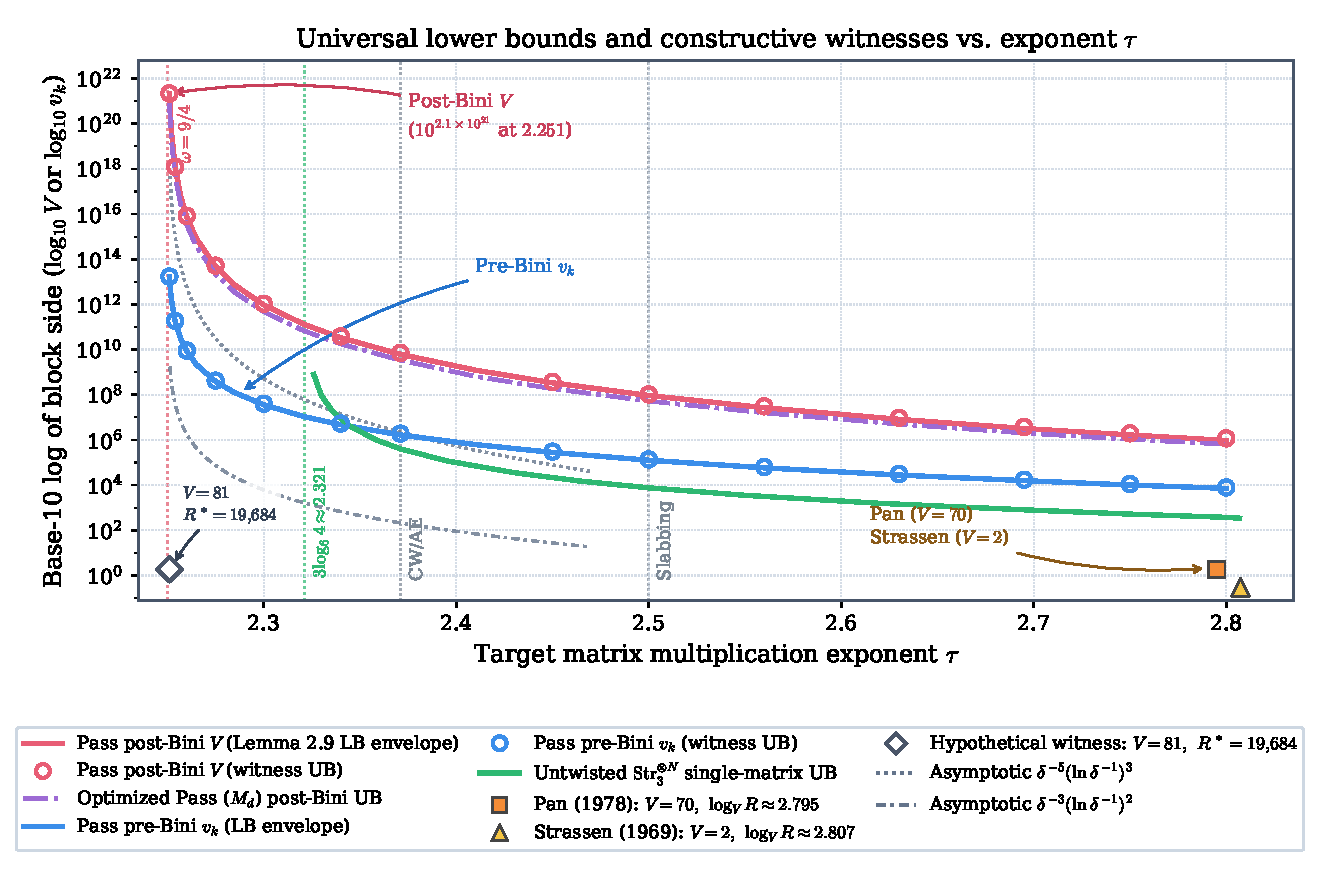
\includegraphics[width=\textwidth]{figures/bounds_vs_exponent.pdf}
\caption{Base-$10$ logarithm of the base block side ($\log_{10} V$ or $\log_{10} v_k$, on a logarithmic vertical scale) vs.\ target matrix multiplication exponent $\tau \in [2.251, 2.807]$. Shown are the universal lower bounds and constructive upper witnesses for Pass's pre-Bini approximate side $v_k$ and post-Bini exact side $V$ (Tables~\ref{tab:pre_bini_bounds}--\ref{tab:post_bini_bounds}), the optimized Pass post-Bini upper bound using exact balanced-word counting $M_d$ and L\"u's $(2w - 1)$-point substitution (Table~\ref{tab:degalactic}), single-shot untwisted $\Str_3^{\otimes N}$ single-matrix achievability stalling at $3\log_6 4 \approx 2.32112$ (Lemma~\ref{lem:finite_schonhage}), classical exact counterexamples by Strassen ($V = 2$) and Pan ($V = 70$; Theorem~\ref{thm:disproof_arbitrary}), the supermultiplicative obstruction witness $(V, R^*) = (16, 513)$ at $\tau = 2.251$ (Theorem~\ref{thm:supermult_obstruction}), and the asymptotic scaling reference curves of Theorem~\ref{thm:asymptotic_scaling}. Generated directly from the exact algebraic recurrences by \texttt{verification/plot\_bounds.py}.}
\label{fig:bounds_vs_exponent}
\end{figure}

\begin{figure}[htbp]
\centering
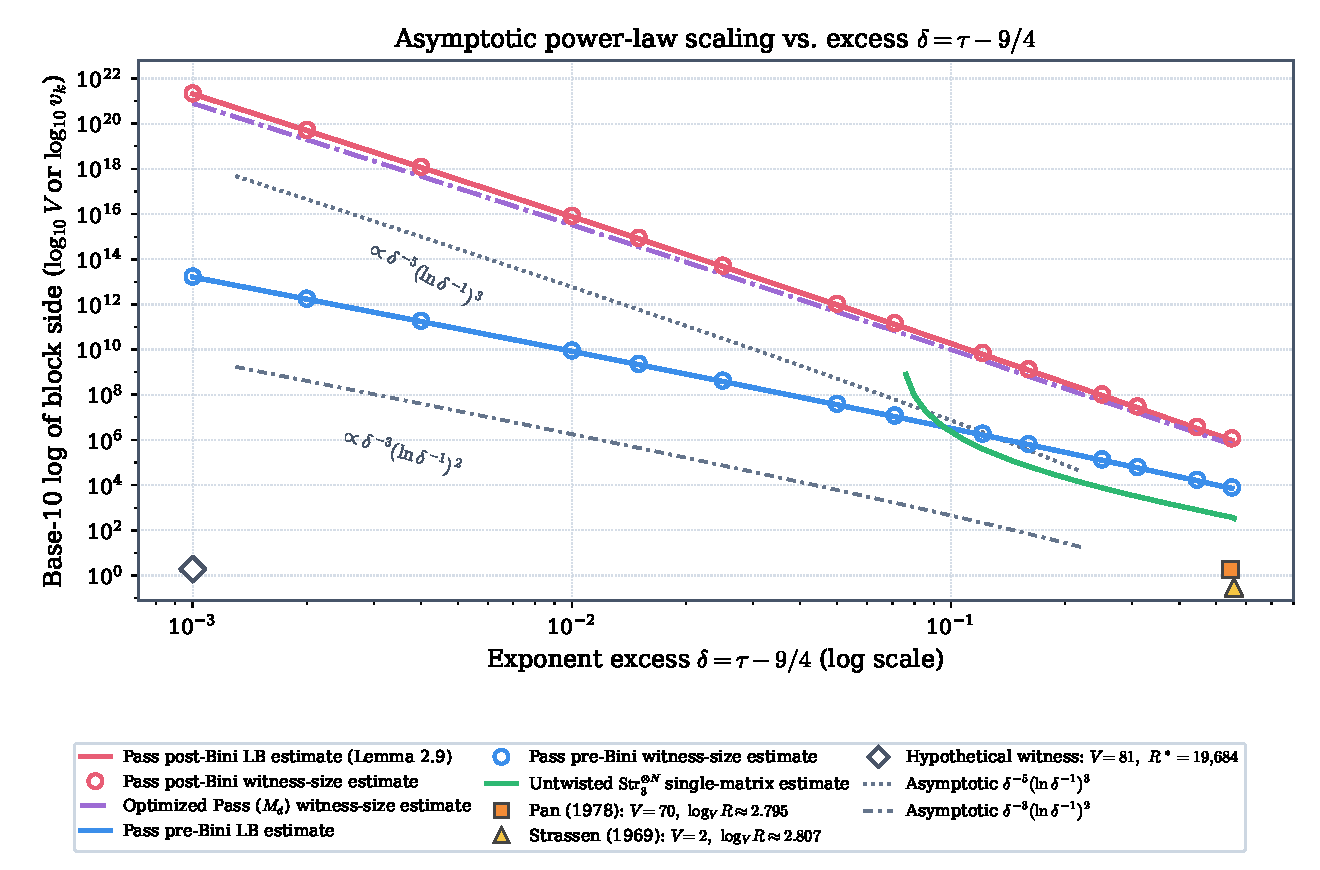
\includegraphics[width=\textwidth]{figures/scaling_vs_excess.pdf}
\caption{Doubly logarithmic power-law scaling of the same universal lower bounds, constructive achievability curves, and witnesses from Figure~\ref{fig:bounds_vs_exponent} plotted against the exponent excess $\delta = \tau - 9/4$. The matched slopes confirm the exact asymptotic laws $\log_{10} v_k = \Theta(\delta^{-3}(\ln\delta^{-1})^2)$ and $\log_{10} V = \Theta(\delta^{-5}(\ln\delta^{-1})^3)$ of Theorem~\ref{thm:asymptotic_scaling} across ten to sixteen orders of magnitude in the double exponent. Generated by \texttt{verification/plot\_bounds.py}.}
\label{fig:scaling_vs_excess}
\end{figure}

%-------------------------------------------------------------------------------
\section{Formal verification in Lean 4}
\label{sec:lean}
%-------------------------------------------------------------------------------

To eliminate floating-point rounding risk and verify every algebraic inequality and numerical bracket over the full infinite parameter domain $(c, d, k, h) \in \N_{\ge 2} \times \N_{\ge 1}^3$, we formalized the results of Sections~\ref{sec:layers} and~\ref{sec:bounds} in pure-kernel Lean~4 inside \texttt{verification/lean/MatMul94/} (using toolchain \texttt{lean4:v4.36.0}, $7{,}559$ lines across five library modules plus root and \texttt{AxiomAudit.lean}) with zero external libraries (no Mathlib), zero \texttt{sorry}, zero custom axioms, and zero \texttt{native\_decide} compiler trust. Every compiled module is independently re-checked via \texttt{leanchecker {-}{-}fresh MatMul94} under \texttt{lake env}, and \texttt{AxiomAudit.lean} certifies via \texttt{\#print axioms} that all $81$ exported headline theorems depend solely on standard Lean foundations (\texttt{propext}, \texttt{Classical.choice}, \texttt{Quot.sound}) or no axioms at all.

Because exact integer evaluations of $v_k \sim 10^{10^{13}}$ or $V \sim 10^{10^{21}}$ cannot be expanded in memory, \texttt{Log2Bracket.lean} implements a compositional dyadic-exponent calculus in \texttt{Nat}:
\begin{equation}
    \mathrm{Log2Ge}(x, p, q) \;\equiv\; \bigl(2^p \le x^q\bigr), \qquad \mathrm{Log2Le}(x, p, q) \;\equiv\; \bigl(x^q \le 2^p\bigr) .
    \label{eq:log2_predicates}
\end{equation}
Under Eq.~\eqref{eq:log2_predicates}, multiplication adds numerators $p_1 + p_2$, raising to any symbolic power $k \in \N$ multiplies the numerator to $k p$ in constant kernel time regardless of the magnitude of $k$, and strict power inequalities $E^q < v^p$ follow directly from linear arithmetic on the numerators. Bridging base~$2$ to base~$10$ via kernel-verified small integer powers ($10^{301} \le 2^{1000} \le 10^{302}$ and $10^{1000} \le 2^{3322}$, $2^{3321} \le 10^{1000}$) converts any dyadic bracket directly into an exact natural-number inequality $10^{M_{\mathrm{lo}}} \le v_k \le 10^{M_{\mathrm{hi}}}$ or $10^{B_{\mathrm{lb}}} < v_k$. Because \texttt{UniversalBounds.lean} closes the infinite quantification over $(c, d, k, h) \in \N^4$ via elementary rational bounds in \texttt{Nat} rather than continuous real-logarithm optimization, its machine-checked universal exponents sit conservatively within $14\%$ to $28\%$ of the continuous sharp lower bounds of Tables~\ref{tab:pre_bini_bounds}--\ref{tab:post_bini_bounds} (for example, $v_k > 10^{6{,}153}$ and $V > 10^{689{,}132}$ at $\tau = 2.800$; $v_k > 10^{1{,}276{,}692}$ and $V > 10^{4.540 \times 10^9}$ at $\tau = 2.371$; $v_k > 10^{1.238 \times 10^{13}}$ and $V > 10^{1.594 \times 10^{21}}$ at $\tau = 2.251$), while proving every inequality with zero floating-point trust.

% Synchronized 1-to-1 with verification/lean/MatMul94/ and AxiomAudit.lean (81 exported theorems, lake build + leanchecker --fresh EC=0).
Table~\ref{tab:lean_map} (Appendix~\ref{app:tables}) records the one-to-one correspondence between the mathematical results of Sections~\ref{sec:layers}--\ref{sec:bounds} and the machine-checked theorems in \texttt{verification/lean/MatMul94/}.

%-------------------------------------------------------------------------------
\section{Conclusion}
\label{sec:conclusion}
%-------------------------------------------------------------------------------

Every layer of the constructive $\omega \le 9/4$ polynomial-packing pipeline contributes a distinct algebraic constraint that forces its hidden constant to astronomical scale. In Layer~1, pure $(c + 1)$-for-$c$ telescoping achieves zero compression (Proposition~\ref{prop:pure_telescoping}), same-slot multi-$\varepsilon$ packing collides on an $\varepsilon^{-1}$ pole (Proposition~\ref{prop:multi_eps_collision}), and the cubic identity $(c + 2)(c - 1)^2 = c^3 - (3c - 2) < c^3$ forces $c > 9/(8\delta) - 3/(4c)$ (Theorem~\ref{thm:cubic_rate_floor}). In Layers~2 through~4, primal-dual balancing in $2d$ variables incurs a logarithmic penalty (Proposition~\ref{prop:balanced_words}), Lagrange uncoupling requires $2w - 1$ evaluations and inner scaling $\eta = \varepsilon^w$ (Proposition~\ref{prop:lagrange_poles}), and the slabbing barrier $3 - \alpha \ge 7/3 > 9/4$ forces three-leg $S_3$-symmetrization and round multiplier $64$ alongside exponential length growth $2 L_k - 1 = \Theta(c\rho^k)$ (Proposition~\ref{prop:slabbing_barrier}, Theorem~\ref{thm:lk_sandwich}). Across all valid parameter triples $(c, d, k)$, these constraints lock the pre-Bini base block side to $\log_{10} v_k(\delta) = \Theta(\delta^{-3}(\ln\delta^{-1})^2)$ (Theorems~\ref{thm:universal_round_and_vk} and~\ref{thm:asymptotic_scaling}), exceeding $10^{7{,}197}$ at $\tau = 2.800$, $10^{1.67 \times 10^6}$ at $\tau = 2.371$, and $10^{1.62 \times 10^{13}}$ at $\tau = 2.251$ (Table~\ref{tab:pre_bini_bounds}). In Layer~5, sequential pole-clearing composition multiplies the $\varepsilon$-degree to $S^{2k} = (3(2d + 1)w - 2)^{2k}$ (Theorem~\ref{thm:pole_cascade}), driving the post-Bini exact base side to $\log_{10} V(\delta) = \Theta(\delta^{-5}(\ln\delta^{-1})^3)$ (exceeding $10^{9.51 \times 10^5}$ at $\tau = 2.800$, $10^{6.15 \times 10^9}$ at $\tau = 2.371$, and $10^{2.08 \times 10^{21}}$ at $\tau = 2.251$) and forcing the arithmetic hidden constant to obey $C(\tau) \ge (V - 1)^{3-\tau}$ even under optimal schoolbook cutoff (Proposition~\ref{prop:hidden_constant}, Table~\ref{tab:post_bini_bounds}). Exact balanced-word counting and L\"u's characteristic-free separation lower $\log_{10} V$ by a constant factor of $1.8$ to $5.9$, while single-shot untwisting of $\Str_3^{\otimes N}$ removes the $2k$-round cascade and reaches sub-Strassen exponent at single-matrix side $10^{343.3}$ ($10^{23.5}$ for a multi-copy direct sum) before stalling at $3\log_6 4 \approx 2.32112$ (Lemma~\ref{lem:finite_schonhage}, Table~\ref{tab:degalactic}).

These lower bounds extend universally to Pass's entire generalized Remark~4.5 iterated polynomial-packing meta-family, where $v_k^{4 a_0} > w^{18 b_0}$ and $d = \Omega(\delta^{-2})$ hold even at zero balancing loss (Theorem~\ref{thm:remark45_universal}), and any border-rank algorithm obeying $r_0 \ge v_0^{9/4}$ obeys the Bini-conversion horizon $V > (h E_\varepsilon + 1)^{1/\delta}$ (Proposition~\ref{prop:general_bini_horizon}). Across arbitrary bilinear algorithms, however, Pass-scale constant lower bounds are disproved for $\tau \in (2.32112, 3)$ by Strassen's $2 \times 2$ identity, Pan's $70 \times 70$ algorithm ($143{,}640^5 < 70^{14}$), and single-shot untwisted $\Str_3^{\otimes N}$ (Theorem~\ref{thm:disproof_arbitrary}). For $\tau \in (9/4, 2.32112)$, every supermultiplicative rank lower bound obeys $\Phi(V) \le V^{9/4}$ and leaves $V = O(\delta^{-4/9})$ (including $V = 16, R = 513$ at $\tau = 2.251$, or exact $R = 512$ at $\delta = 0$) consistent with $\omega_{\F} = 9/4$ (Theorem~\ref{thm:supermult_obstruction}).

Two concrete mathematical problems remain open. The first is whether any constant-round ($k = O(1)$) degeneration sequence achieves exponents arbitrarily close to $9/4$, which would bypass the $2k$-round pole-clearing cascade and reduce $\log_{10} V(\delta)$ below $\Theta(\delta^{-5}(\ln\delta^{-1})^3)$. The second is whether any non-supermultiplicative finite-size lower bound proves $R(\langle V, V, V\rangle) \ge V^{9/4+\delta}$ across a super-polynomial range of base sides $V$ for $\tau \in (9/4, 2.32112)$, or conversely whether a small exact bilinear identity outside the iterated polynomial-packing family (such as $V = 16, R \le 513$) exists.

\appendix

\begin{landscape}
%-------------------------------------------------------------------------------
\section{Summary tables}
\label{app:tables}
%-------------------------------------------------------------------------------

Tables~\ref{tab:separations}--\ref{tab:lean_map} collect the shared-leg separation comparison, pre-Bini and post-Bini quantitative brackets, de-galacticization benchmarks, and pure-kernel Lean~4 theorem correspondence in landscape orientation.

\begin{table}[!htbp]
\centering
\small
\caption{Comparison of the four shared-leg separation constructions for $M$ matched blocks (with $n = M$ auxiliary dot-product dimension; $M = w$ in Pass's Lemma~3.4). The exact $\varepsilon$-degree for OpenAI's $5M$ scheme is established by Proposition~\ref{prop:openai_5m_tight}.}
\label{tab:separations}
\begin{tabular}{@{} l c l c @{}}
\toprule
\textbf{Construction} & \textbf{Source copies} & \textbf{Field requirement} & \textbf{Exact $\varepsilon$-degree} \\
\midrule
OpenAI~\cite[Prop.~3.1]{OpenAI2026Upper} & $5M$ & $\mathrm{char}(\F) \nmid 5M$, primitive $\zeta_{5M}$ & $\lfloor (M - 1)/2 \rfloor^2$ \\
Uzna\'nski~\cite[App.~C]{Uznanski2026} & $2M$ & $\mathrm{char}(\F) \nmid 2M$, primitive $\zeta_{2M}$ & $(M - 1)^2$ \\
Pass~\cite[Lemma~3.4]{Pass2026} & $2M - 1$ & $\mathrm{char}(\F) = 0$ (rational nodes) & $M - 1$ (outer pole) \\
L\"u~\cite[Prop.~2.1]{Lu2026} & $2M - 1$ & Arbitrary char., $|\F| \ge 2M - 1$ & $M - 1$ \\
\bottomrule
\end{tabular}
\end{table}

\begin{table}[!htbp]
\centering
\small
\caption{Pre-Bini approximate base block side $v_k = w^2 \Lambda^k$ in Pass's Theorem~4.3 across eight target exponents $\tau$. The universal lower bound holds for every Pass-valid triple $(c, d, k) \in \N_{\ge 2} \times \N_{\ge 1} \times \N_{\ge 1}$ via Eqs.~\eqref{eq:sharp_denom}--\eqref{eq:sharp_k_lnLam_lb}; the constructive upper witness $(c^*, d^*, k^*)$ evaluates the exact recurrence Eq.~\eqref{eq:Lk_recurrence} and satisfies Eq.~\eqref{eq:pass_valid_cond}.}
\label{tab:pre_bini_bounds}
\begin{tabular}{@{} l c r r c c @{}}
\toprule
\textbf{Target $\tau$ (benchmark)} & $c_{\min}(\tau)$ & \textbf{Univ.\ LB $\log_{10} v_k >$} & \textbf{Constructive UB $\log_{10} v_k$} & \textbf{Witness $(c^*, d^*, k^*)$} & \textbf{UB / LB} \\
\midrule
$2.800$ (sub-Strassen) & $3$ & $7{,}197.27$ & $7{,}927.63$ & $(6,\; 139,\; 114)$ & $1.101$ \\
$2.695$ ($P_{2,4}$ threshold) & $3$ & $15{,}809.49$ & $17{,}442.54$ & $(6,\; 207,\; 169)$ & $1.103$ \\
$2.500$ (sub-slabbing) & $5$ & $126{,}725.43$ & $137{,}617.22$ & $(12,\; 719,\; 719)$ & $1.086$ \\
$2.371$ (sub-CW / AlphaEvolve) & $10$ & $1{,}671{,}405.33$ & $1{,}770{,}235.12$ & $(24,\; 3{,}392,\; 3{,}769)$ & $1.059$ \\
$2.321$ (untwisted $\Str_3$) & $17$ & $10{,}782{,}969.44$ & $11{,}348{,}489.01$ & $(42,\; 10{,}917,\; 12{,}900)$ & $1.052$ \\
$2.300$ & $23$ & $36{,}254{,}552.34$ & $37{,}963{,}961.01$ & $(57,\; 23{,}003,\; 27{,}605)$ & $1.047$ \\
$2.260$ & $113$ & $8.439 \times 10^{9}$ & $8.719 \times 10^{9}$ & $(304,\; 763{,}002,\; 1{,}003{,}639)$ & $1.033$ \\
$2.251$ & $1{,}126$ & $1.625 \times 10^{13}$ & $1.661 \times 10^{13}$ & $(3{,}032,\; 1.026 \times 10^8,\; 1.413 \times 10^8)$ & $1.022$ \\
\bottomrule
\end{tabular}
\end{table}

\clearpage

\begin{table}[!htbp]
\centering
\small
\caption{Post-Bini exact base block side $V = v_{k_b}^h$ under Pass's sequential pole-clearing composition (Theorem~\ref{thm:pole_cascade}) and implied lower bounds on the arithmetic hidden constant $C(\tau)$ (Proposition~\ref{prop:hidden_constant}: schoolbook cutoff $C_{\mathrm{sb}} \ge (V - 1)^{3-\tau}$, Strassen cutoff $C_{\mathrm{Str}} \ge ((V - 1)/2)^{\log_2 7 - \tau}$, and power-of-$V$ padding $C_{\mathrm{pad}} \ge V^4/(V + 1)^\tau$).}
\label{tab:post_bini_bounds}
\begin{tabular}{@{} l c c c c c c @{}}
\toprule
\textbf{$\tau$} & \textbf{Post LB $\log_{10} V >$} & \textbf{Post UB $\log_{10} V$} & \textbf{Witness $(c, d, k_b, h)$} & \textbf{$\log_{10} C_{\mathrm{sb}} >$} & \textbf{$\log_{10} C_{\mathrm{Str}} >$} & \textbf{$\log_{10} C_{\mathrm{pad}} >$} \\
\midrule
$2.800$ & $9.510 \times 10^{5}$ & $1.173 \times 10^{6}$ & $(5,\; 219,\; 150,\; 61)$ & $1.902 \times 10^{5}$ & $6.995 \times 10^{3}$ & $1.141 \times 10^{6}$ \\
$2.695$ & $3.215 \times 10^{6}$ & $3.755 \times 10^{6}$ & $(6,\; 335,\; 236,\; 95)$ & $9.806 \times 10^{5}$ & $3.612 \times 10^{5}$ & $4.196 \times 10^{6}$ \\
$2.500$ & $9.306 \times 10^{7}$ & $1.046 \times 10^{8}$ & $(10,\; 1{,}073,\; 866,\; 356)$ & $4.653 \times 10^{7}$ & $2.860 \times 10^{7}$ & $1.396 \times 10^{8}$ \\
$2.371$ & $6.151 \times 10^{9}$ & $6.726 \times 10^{9}$ & $(21,\; 5{,}052,\; 4{,}756,\; 1{,}775)$ & $3.869 \times 10^{9}$ & $2.684 \times 10^{9}$ & $1.002 \times 10^{10}$ \\
$2.321$ & $1.304 \times 10^{11}$ & $1.403 \times 10^{11}$ & $(36,\; 16{,}021,\; 16{,}123,\; 5{,}793)$ & $8.854 \times 10^{10}$ & $6.342 \times 10^{10}$ & $2.189 \times 10^{11}$ \\
$2.300$ & $9.564 \times 10^{11}$ & $1.020 \times 10^{12}$ & $(51,\; 34{,}246,\; 35{,}518,\; 12{,}558)$ & $6.695 \times 10^{11}$ & $4.852 \times 10^{11}$ & $1.626 \times 10^{12}$ \\
$2.260$ & $7.658 \times 10^{15}$ & $7.985 \times 10^{15}$ & $(255,\; 1.107 \times 10^6,\; 1.253 \times 10^6,\; 4.243 \times 10^5)$ & $5.667 \times 10^{15}$ & $4.192 \times 10^{15}$ & $1.332 \times 10^{16}$ \\
$2.251$ & $2.082 \times 10^{21}$ & $2.145 \times 10^{21}$ & $(2{,}546,\; 1.490 \times 10^8,\; 1.787 \times 10^8,\; 5.904 \times 10^7)$ & $1.559 \times 10^{21}$ & $1.158 \times 10^{21}$ & $3.641 \times 10^{21}$ \\
\bottomrule
\end{tabular}
\end{table}

\begin{table}[!htbp]
\centering
\footnotesize
\caption{Post-Bini base block side $\log_{10} V$ across four constructions: OpenAI $5w$ separation in Pass's $2k$-round pipeline, literal Pass ($2w$, Cauchy--Schwarz $d + 1$), optimized Pass (L\"u/Pass $2w - 1$ with exact balanced-word count $M_d$), and single-shot untwisted $\Str_3^{\otimes N}$ with L\"u $2M - 1$ separation (reporting both the multi-copy direct-sum side $v_{\mathrm{Str}}^{h_{\mathrm{Str}}}$ for $P_{\mathrm{Str}} = M^{3 h_{\mathrm{Str}}}$ copies and the single-matrix side $V_{\mathrm{single}} = v_{\mathrm{Str}}^{h_{\mathrm{Str}} r_{\mathrm{Sch}}}$ via Lemma~\ref{lem:finite_schonhage}; floor $3\log_6 4 \approx 2.32112$).}
\label{tab:degalactic}
\begin{tabular}{@{} l c c c c c @{}}
\toprule
\textbf{Target $\tau$} & \textbf{OpenAI $5w$} & \textbf{Literal Pass} & \textbf{Opt.\ Pass ($M_d$)} & \textbf{$\Str_3$ Direct Sum ($P_{\mathrm{Str}}$)} & \textbf{$\Str_3$ Single Matrix} \\
\midrule
$2.800 / 2.807$ (Strassen) & $2.810 \times 10^{6}$ & $1.173 \times 10^{6}$ & $6.476 \times 10^{5}$ & $23.49$ ($P_{\mathrm{Str}} = 10^{24.66}$) & $343.25$ ($N{=}22, h_{\mathrm{Str}}{=}3, r_{\mathrm{Sch}}{=}7$) \\
$2.695$ ($P_{2,4}$) & $8.929 \times 10^{6}$ & $3.755 \times 10^{6}$ & $2.032 \times 10^{6}$ & $39.82$ ($P_{\mathrm{Str}} = 10^{42.18}$) & $810.15$ ($N{=}30, h_{\mathrm{Str}}{=}4, r_{\mathrm{Sch}}{=}9$) \\
$2.500$ (Slabbing) & $2.426 \times 10^{8}$ & $1.046 \times 10^{8}$ & $5.319 \times 10^{7}$ & $174.32$ ($P_{\mathrm{Str}} = 10^{193.73}$) & $7{,}629.06$ ($N{=}68, h_{\mathrm{Str}}{=}7, r_{\mathrm{Sch}}{=}21$) \\
$2.371$ (CW / AE) & $1.530 \times 10^{10}$ & $6.726 \times 10^{9}$ & $3.182 \times 10^{9}$ & $2{,}492.38$ ($P_{\mathrm{Str}} = 10^{2{,}854}$) & $4.047 \times 10^{5}$ ($N{=}272, h_{\mathrm{Str}}{=}26, r_{\mathrm{Sch}}{=}74$) \\
$2.330$ & N/A & N/A & N/A & $94{,}489.26$ ($P_{\mathrm{Str}} = 10^{109{,}380}$) & $9.371 \times 10^{7}$ ($N{=}1{,}498, h_{\mathrm{Str}}{=}166, r_{\mathrm{Sch}}{=}485$) \\
$2.260$ & $1.737 \times 10^{16}$ & $7.985 \times 10^{15}$ & $3.178 \times 10^{15}$ & unreachable ($< 2.32112$) & unreachable ($< 2.32112$) \\
$2.251$ & $4.570 \times 10^{21}$ & $2.145 \times 10^{21}$ & $7.762 \times 10^{20}$ & unreachable ($< 2.32112$) & unreachable ($< 2.32112$) \\
\bottomrule
\end{tabular}
\end{table}

\clearpage

\begin{table}[!htbp]
\centering
\footnotesize
\caption{Correspondence between paper theorems and pure-kernel Lean~4 theorems in \texttt{verification/lean/MatMul94/} ($7{,}559$ lines, $81$ exported theorems audited in \texttt{AxiomAudit.lean}, zero Mathlib, zero \texttt{sorry}, zero \texttt{native\_decide}, verified by \texttt{lake env leanchecker {-}{-}fresh MatMul94}).}
\label{tab:lean_map}
\begin{tabular}{@{} >{\raggedright\arraybackslash}p{6.6cm} l >{\raggedright\arraybackslash}p{12.6cm} @{}}
\toprule
\textbf{Paper result} & \textbf{Lean module} & \textbf{Verified Lean theorem(s)} \\
\midrule
Eq.~\eqref{eq:log2_predicates} (dyadic calculus \& $10^{301} \le 2^{1000} \le 10^{302}$) & \texttt{Log2Bracket.lean} & \texttt{pow10\_301\_le\_pow2\_1000}, \texttt{add\_two\_pow\_lt\_eight} \\
Prop.~\ref{prop:pure_telescoping} (zero-gain telescoping) & \texttt{LayerConstraints.lean} & \texttt{pure\_telescoping\_zero\_gain} \\
Thm.~\ref{thm:primal_gap} (zero-gap identity \& surplus) & \texttt{LayerConstraints.lean} & \texttt{primal\_telescoping\_identity}, \texttt{gap\_window\_disjoint}, \texttt{effort\_surplus\_positive} \\
Prop.~\ref{prop:multi_eps_collision} (same-slot pole collision) & \texttt{LayerConstraints.lean} & \texttt{same\_slot\_multi\_eps\_collision} \\
Thm.~\ref{thm:cubic_rate_floor} (cubic rate floor $> 9/4$ \& $c_{\min}$) & \texttt{LayerConstraints.lean} & \texttt{cubic\_rate\_gap}, \texttt{pass\_rate\_strictly\_above\_9\_4}, \texttt{c\_min\_polynomial\_bound} \\
Prop.~\ref{prop:balanced_words} (balanced-word bounds) & \texttt{LayerConstraints.lean} & \texttt{cauchy\_schwarz\_balanced\_words} \\
Prop.~\ref{prop:lagrange_poles} \&~\ref{prop:openai_5m_tight} (Lagrange \& $5M$ deg.) & \texttt{LayerConstraints.lean} & \texttt{lagrange\_uncoupling\_constraints}, \texttt{inner\_eta\_pole\_clearing\_necessity}, \texttt{openai\_5M\_tight\_eps\_deg} \\
Prop.~\ref{prop:slabbing_barrier} \& Thm.~\ref{thm:lk_sandwich} (slabbing \& $L_k$) & \texttt{LayerConstraints.lean} & \texttt{slabbing\_barrier}, \texttt{exact\_Lk\_sandwich} \\
Thm.~\ref{thm:pole_cascade}, Prop.~\ref{prop:hidden_constant}, Lemma~\ref{lem:finite_schonhage} & \texttt{LayerConstraints.lean} & \texttt{pole\_cascade\_exact}, \texttt{multivariate\_bini\_worse}, \texttt{hidden\_constant\_bounds}, \texttt{finite\_schonhage} \\
Thm.~\ref{thm:universal_round_and_vk} (pure-integer universal bounds) & \texttt{UniversalBounds.lean} & \texttt{universal\_round\_necessary}, \texttt{w18\_vk9\_lt\_Ek4}, \texttt{universal\_vk\_pow\_gt\_w\_pow} \\
Tables~\ref{tab:pre_bini_bounds}--\ref{tab:post_bini_bounds} ($c_{\min}$, pre/post universal LBs) & \texttt{UniversalBounds.lean} & \texttt{universal\_c\_min\_all}, \texttt{universal\_vk\_lb\_2807}..\texttt{2251}, \texttt{universal\_post\_bini\_lb\_2807}..\texttt{2251} \\
Tables~\ref{tab:pre_bini_bounds}--\ref{tab:degalactic} (constructive witnesses) & \texttt{ConstructiveWitnesses.lean} & \texttt{witness\_pre\_2800}..\texttt{2251}, \texttt{witness\_post\_2800}..\texttt{2251}, \texttt{witness\_str3\_*} \\
Thm.~\ref{thm:remark45_universal} \& Prop.~\ref{prop:general_bini_horizon} (Remark~4.5 \& Bini) & \texttt{GeneralLimits.lean} & \texttt{remark45\_universal\_round\_necessary}, \texttt{remark45\_universal\_vk\_pow\_gt\_w\_pow}, \texttt{general\_bini\_deg\_horizon} \\
Thm.~\ref{thm:disproof_arbitrary} (arbitrary-algorithm disproof) & \texttt{GeneralLimits.lean} & \texttt{counterexample\_strassen\_1969}, \texttt{counterexample\_pan\_1978}, \texttt{counterexample\_str3\_beats\_pass\_*} \\
Thm.~\ref{thm:supermult_obstruction} (supermultiplicative obstruction) & \texttt{GeneralLimits.lean} & \texttt{supermultiplicative\_bound\_le\_9\_4}, \texttt{bernoulli\_add\_one\_lt\_two}, \texttt{small\_V\_consistent\_with\_9\_4\_general}, \texttt{small\_V\_16\_witness\_2251} \\
\bottomrule
\end{tabular}
\end{table}

\clearpage

%-------------------------------------------------------------------------------
\section{Notation}
\label{app:notation}
%-------------------------------------------------------------------------------

Table~\ref{tab:notation} lists the principal symbols of the paper, grouped by the section in which each symbol is first defined. Standard sets ($\N, \Z, \Q, \R, \C$) and local summation or iteration indices ($i, j, \ell, r$) are omitted.

{\small
\begin{longtable}{@{} l >{\raggedright\arraybackslash}p{13.8cm} l @{}}
\caption{Principal symbols grouped by section of first definition.}
\label{tab:notation} \\
\toprule
\textbf{Symbol} & \textbf{Meaning} & \textbf{Definition} \\
\midrule
\endfirsthead
\toprule
\textbf{Symbol} & \textbf{Meaning} & \textbf{Definition} \\
\midrule
\endhead
\midrule
\multicolumn{3}{r}{\textit{Continued on next page}} \\
\endfoot
\bottomrule
\endlastfoot
\multicolumn{3}{@{}l}{\textbf{Section~\ref{sec:intro} (Introduction)}} \\
$\omega_{\F}$ & Square matrix multiplication exponent over field $\F$ & Sec.~\ref{sec:intro} \\
$\alpha_{\F}$ & Dual rectangular matrix multiplication exponent ($\omega_{\F}(1, \alpha, 1) = 2$) & Sec.~\ref{sec:intro} \\
$\tau, \delta$ & Target exponent $\tau > 9/4$ and excess $\delta = \tau - 9/4$ & Sec.~\ref{sec:intro} \\
$\Str_3$ & Strassen three-variable tensor $\langle 3, 1, 1\rangle \oplus_3 \langle 1, 1, 3\rangle$ (border rank $4$) & Sec.~\ref{sec:intro} \\
$v_k, V$ & Pre-Bini approximate and post-Bini exact base block side lengths & Sec.~\ref{sec:intro} \\
$C(\tau)$ & Hidden multiplicative constant in $T(n) \le C(\tau)\,n^\tau$ & Sec.~\ref{sec:intro} \\
\midrule
\multicolumn{3}{@{}l}{\textbf{Section~\ref{sec:setup} (Bilinear algorithms and polynomial packings)}} \\
$\nu$ & Number of polynomial indeterminates $z = (z_1, \dots, z_\nu)$ & Sec.~\ref{sec:setup} \\
$\Prod_{I,J,K}[p,q,r]$ & Selected matrix-polynomial product of shape $(I, J, K)$ & Eq.~\eqref{eq:selected_product} \\
$\langle p, q, r\rangle$ & Matrix multiplication tensor of sizes $(p \times q) \times (q \times r)$ & Sec.~\ref{sec:setup} \\
$\Full_{a,b}, \Mid_{a,b}$ & Univariate full-product and middle-product shapes of lengths $a, b$ ($s = a + b - 1$) & Eqs.~\eqref{eq:full_shape}--\eqref{eq:mid_shape} \\
$\eff(P[p,q,r])$ & Evaluation effort of selected product $P[p,q,r]$ & Eq.~\eqref{eq:effort_def} \\
$E^L, E^R, D$ & Left encoder, right encoder, and decoder of a polynomial packing & Eq.~\eqref{eq:exact_pp} \\
$R, \underline{R}$ & Exact bilinear rank and approximate border rank & Def.~\ref{def:packing} \\
$p_L, p_R, p_D, d_\varepsilon$ & Encoder/decoder pole orders and output degree in $\varepsilon$ & Sec.~\ref{sec:setup} \\
\midrule
\multicolumn{3}{@{}l}{\textbf{Section~\ref{sec:layers} (Algebraic constraints)}} \\
$c, t$ & Packing parameter ($c \ge 2$) and shift width ($ct \ge a + 2b - 1$) & Eq.~\eqref{eq:gap_condition} \\
$\rho(c), \tau(c)$ & Round length-inflation factor $(c + 2)/(c - 1)$ and asymptotic exponent threshold & Eqs.~\eqref{eq:rho_def}--\eqref{eq:tau_c_def} \\
$d, u(c, d)$ & Half-variable count ($2d$ variables per leg) and source count $c^{2d}$ & Eq.~\eqref{eq:u_def} \\
$M_d(c), w(c, d)$ & Exact balanced-word count and Cauchy--Schwarz floor $\lfloor (c+2)^{2d}/(d+1)\rfloor$ & Eqs.~\eqref{eq:Md_exact}, \eqref{eq:w_def} \\
$p_b$ & Binomial parameter $(c + 2)^{-1}$ in $M_d(c)$ asymptotic formula & Eq.~\eqref{eq:Md_stirling} \\
$\eta, M$ & Inner SL-PP parameter ($\eta = \varepsilon^w$) and shared-leg matched block count & Props.~\ref{prop:lagrange_poles}, \ref{prop:openai_5m_tight} \\
$P_1, N_1$ & Single-leg Layer~3 pole-order sum and maximum positive $\varepsilon$-degree & Eq.~\eqref{eq:single_leg_poles} \\
$\Lambda(c, d)$ & Per-round side-length multiplier $\lfloor w/u \rfloor^2$ & Eq.~\eqref{eq:lambda_def} \\
$k, L_k(c), j_0$ & Round count, ceiling length recurrence, and boost threshold $\lfloor (c - 1)/3 \rfloor$ & Eq.~\eqref{eq:Lk_recurrence}, Thm.~\ref{thm:lk_sandwich} \\
$E_k(c, d)$ & Pre-Bini approximate scalar multiplication count $64^k w^9 (2 L_k - 1)^{6d}$ & Eq.~\eqref{eq:Ek_def} \\
$P_{\mathrm{half}}, N_{\mathrm{half}}, S, D_{\mathrm{half}}$ & Half-round pole sum, max positive degree, substitution multiplier $P_{\mathrm{half}} + 1$, per-half-round degree & Eq.~\eqref{eq:half_round_poles}, Thm.~\ref{thm:pole_cascade} \\
$h, R_{\mathrm{exact}}$ & Bini tensor power ($V = v_k^h$) and post-Bini exact bilinear rank & Eqs.~\eqref{eq:V_post_def}--\eqref{eq:R_exact_def} \\
$C_{\mathrm{sb}}, C_{\mathrm{Str}}, C_{\mathrm{pad}}$ & Hidden-constant lower bounds under schoolbook, Strassen, and power-of-$V$ padding & Eqs.~\eqref{eq:C_schoolbook}--\eqref{eq:C_padding} \\
\midrule
\multicolumn{3}{@{}l}{\textbf{Section~\ref{sec:bounds} (Universal lower bounds and constructive witnesses)}} \\
$p_\tau, q_\tau, a_0, b_0$ & Exact rational target integers $\tau = p_\tau / q_\tau = 9/4 + a_0/b_0$ & Eq.~\eqref{eq:pass_valid_cond} \\
$\lambda_{\mathrm{ub}}, \Delta_{\mathrm{ub}}$ & Exact upper bounds on $\ln\Lambda$ and per-round exponent margin & Eq.~\eqref{eq:sharp_denom} \\
$N, h_{\mathrm{Str}}, r_{\mathrm{Sch}}$ & Untwisted $\Str_3^{\otimes N}$ power, Bini power, and finite Sch\"onhage power & Sec.~\ref{subsec:degalactic}, Lemma~\ref{lem:finite_schonhage} \\
$m_{\mathrm{t}}, n_{\mathrm{s}}, R_{\mathrm{num}}, R_{\mathrm{den}}, \Delta_{\mathrm{bal}}$ & Remark~4.5 target/source counts, rational effort factor $\rho_0^\kappa$, and balancing denominator & Thm.~\ref{thm:remark45_universal} \\
$v_0, r_0, E_\varepsilon$ & General border-rank identity side, border rank, and output $\varepsilon$-degree & Prop.~\ref{prop:general_bini_horizon} \\
$\Phi, \mu, R^*$ & Supermultiplicative rank lower bound and polynomial-size consistency witness $(\mu^4, \mu^9 + 1)$ & Thm.~\ref{thm:supermult_obstruction} \\
\midrule
\multicolumn{3}{@{}l}{\textbf{Section~\ref{sec:lean} (Formal verification in Lean 4)}} \\
$\mathrm{Log2Ge}, \mathrm{Log2Le}$ & Pure-kernel dyadic-exponent predicates $2^p \le x^q$ and $x^q \le 2^p$ & Eq.~\eqref{eq:log2_predicates} \\
\end{longtable}
}
\end{landscape}

\bibliographystyle{plain}
\bibliography{matmul_9_4_constant}

\end{document}
